\documentclass{sig-alternate}

\usepackage{latexsym}
\usepackage{amsmath}
\usepackage{color}
\usepackage{graphicx}
\usepackage{amssymb}
\usepackage{epstopdf}
\usepackage{algorithmic}
\DeclareGraphicsRule{.tif}{png}{.png}{`convert #1 `dirname #1`/`basename #1 .tif`.png}



\def\punto{$\hspace*{\fill}\Box$}
\newcommand{\nop}[1]{}
\newcommand{\tuple}[1]{{\langle#1\rangle}}
\def\lBrack{\lbrack\!\lbrack}
\def\rBrack{\rbrack\!\rbrack}
\newcommand{\Bracks}[1]{\lBrack#1\rBrack}


\newtheorem{theorem}{Theorem}[section]
\newtheorem{proposition}[theorem]{Proposition}
\newtheorem{example}[theorem]{Example}
\newtheorem{remark}[theorem]{Remark}

\nop{
\newtheorem{metatheorem}{Metatheorem}[section]
\newtheorem{algorithm}[theorem]{Algorithm}
\newtheorem{definition}[theorem]{Definition}
\newtheorem{property}[theorem]{Property}
\newtheorem{corollary}[theorem]{Corollary}
\newtheorem{lemma}[theorem]{Lemma}
\newtheorem{conjecture}[theorem]{Conjecture}
\newtheorem{proviso}[theorem]{Proviso}
\newtheorem{todo}[theorem]{ToDo}
} % end nop




\conferenceinfo{SIGMOD}{'10 Indianapolis, IN}


%\title{The Cumulus System for Exact Online Aggregation in the Cloud}
%\title{Cumulus: A Distributed Exact Online Aggregation System}
%\title{Cumulus: Exact Online Aggregation by Message Passing}
\title{Exact Online Aggregation by Message Passing}


\numberofauthors{3}
\author{}%Oliver Kennedy, Yanif Ahmad, Christoph Koch}
\toappear{}


\begin{document}

\maketitle


\abstract{
We present Cumulus, a distributed exact online aggregation system.
Cumulus compiles a set of SQL aggregation queries
%
% or a datacube
%
down to a message-passing program that incrementally maintains
the query results by simple and highly efficient local modifications.
Surprisingly, for each tuple inserted, updated, or deleted,
our message passing programs
have to perform only a {\em constant}\/ amount of work per
aggregate value to be maintained.
%
%assuming constant-time read/write access to individual data items.
%This can be guaranteed if the data is kept in main memory.
%
Our message-passing protocol also allows for massive parallelization.

The Cumulus runtime system is a distributed key-value store for
aggregate-group-by query results that implements our message passing protocol
for incremental result maintenance.
Cumulus efficiently answers OLAP queries using this store.
Cumulus performs the incremental maintenance of large views under
considerable update loads in realtime, leveraging parallelism
and using the resources of the cloud to keep its store in main memory.
}



It is immediately plausible that one can do better than re-evaluate a query from scratch whenever the database changes a little. Incremental view maintenance (IVM) capitalizes on this insight \cite{DBLP:journals/tods/BunemanC79,DBLP:conf/sigmod/ShmueliI84,DBLP:conf/sigmod/BlakeleyLT86,roussopoulos-tods:91,DBLP:conf/vldb/CeriW91,DBLP:conf/deductive/GuptaKM92,DBLP:conf/sigmod/GuptaMS93,griffin-sigmod:95,yan-vldb:95,colby-sigmod:96,GHJ1996,kotidis-tods:01}. It is a solid, settled technique that has been implemented in many commercial DBMS, but has seen little new research activity in recent years and has gathered a little dust.

Now there is an exciting and potentially game-changing new development \cite{ahmad-vldb:09, koch-pods:10, kennedy-ahmad-koch-cidr:11}, an extreme form of IVM where all query evaluation work reduces to adding data (updates or materialized query results) to other materialized query results.  No join processing or anything semantically equivalent happens at any stage of processing. This works for a fragment of SQL with equijoins and aggregation, but without inequality joins or nesting aggregates.


Let us digest this, because the last claim goes counter to query processing intuitions to the point of absurdity. The main idea is the following: Classical IVM revolves around the idea that a materialized view can be maintained under updates by evaluating a so-called delta query and adding its result to the materialized view. The delta query captures how the query result changes in response to a change in the database. The new observation is that the delta query can be materialized and incrementally maintained using the same idea, making use of a delta query to the delta query, which again can be materialized and incrementally maintained, and so on, recursively. This works for classes of queries whose deltas are in some way structurally simpler than the base queries (e.g. having fewer joins), allowing this recursive query transformation to terminate. (It does so with a final trivial $k$-th delta query that does not refer to the database at all.) Termination is ensured for select-project-join queries with certain forms of aggregation, but some other features of SQL (specifically aggregations nested in where-conditions) have to be excluded. 

So where do the joins go? They {\em really} go away, as a benefit of incremental computation. If we want to compute $(x+1)*y$ and know $x*y$ and $y$, we only need to add $y$ to $x*y$, and the multiplication goes away. This is what happens when incrementally maintaining a join, where the join takes the place of multiplication. The pattern just sketched in basic algebra is not just an intuition but exactly what happens, and \cite{koch-pods:10} develops the algebraic framework to formalize this. We observe that the symbol 1 above represents the update workload.  In the incremental query processing framework, it must be a {\em constant} number of tuples that are changed in each incrementation step.

\comment{
To the reader who still cannot accept that joins can be replaced by no joins, we observe that the history of all incremental updates to the materialized view taken together is still essentially an execution of a nested loops join, that is, overall the value $x*y$ is constructed by adding $x$ copies of $y$. So if we put all the work associated with the individual updates happening over time together, the join work is still done. But refreshing the view in response to a single update does not require joins.
}

On paper, this approach clearly dominates classical IVM: if classical IVM is a good idea, then doing it recursively is an even better idea: The same efficiency-improvement argument for incremental maintenance of the base query also applies to the delta query. Argued from the viewpoint that joins are expensive and this approach eliminates them, one should expect a potential for excellent query performance.

But does this expectation translate into real performance gains? A priori, the cost of the bulk addition of materialized views or the costs associated with storing and managing additional auxiliary materialized views (for delta queries) might be more considerable than expected.


\medskip


This paper presents the lessons learned in an effort to realize recursive IVM, spanning nearly three years of intense work, to generalize it to be applicable on all or most of SQL, and to understand its strengths and drawbacks.
The contributions of this paper are as follows.
\begin{itemize}
\item
Multilevel IVM bears the promise of providing materialized views of complex SQL queries, without
window semantics or other restrictions, at very high refresh rates. We start by showing that there is
a need for such functionality, creating a benchmark consisting of automated trading and ETL workloads.
We show that state of the art systems cannot deliver materialized views refreshed at the rates
that some application domains (algorithmic trading, real-time analytics) require.
This is the challenge we set ourselves for the techniques and system described in this paper.

\item
We develop the vision of multilevel IVM further into a workable system.
While the techniques of \cite{ahmad-vldb:09, koch-pods:10} as well as existing implementations of
IVM in commercial DBMS are very restricted and exclude nested queries and other features of SQL,
we create the machinery to perform IVM and even recursive IVM on most of SQL (with the exception of
support for null values). To do this, we generalize the techniques of \cite{ahmad-vldb:09, koch-pods:10}
to not always materialize full delta queries but instead subexpressions that allow us to perform
IVM and maximize the performance obtained. This leads us to a query optimizer in which
the materialization of subqueries is a degree of freedom in optimization, and can be applied anywhere
in the input query or the delta queries obtained by applying this optimization.

To put ourselves in the position of using such an optimizer, we have to create suitable
intermediate representations of queries that support binding patterns for sideways information
passing, we study when and how to efficiently initialize views, and present query decomposition
and factorization techniques that lead to efficient formulations of update triggers that refresh our
views.

\item
Once high-level trigger programs for refreshing views based on multilevel IVM have been created,
we compile them further into highly efficient machine code.
We present our techniques for achieving this, which make use of sophisticated deforestation and
fusion techniques from the compilers literature.

\item
We have implemented our compiler and performed extensive experimentation with it. Our experiments
indicate that frequently, particularly for queries that consist of many joins of nested aggregation
subqueries that are not correlated through subqueries, our compilation approach dominates the
state of the art, often by multiple orders of magnitude. There are also queries in our benchmark
on which our techniques do not fare well; these usually involve the creation and maintenance of huge
auxiliary views whose data is rarely used by other views. These scenarios could be much improved upon
by suitable garbage collection strategies on auxiliary views. This is future work, and we consider
it likely that once such a technique has been integrated into our compiler, it will outperform the
state-of-the-art on an even wider range of queries.
\end{itemize}


The structure of the paper follows the order of contribution just laid out.















\comment{
This paper presents the lessons learned in an effort to realize aggressive IVM as motivated above. It represents an effort spanning nearly three years of intense work, which demonstrates that there are considerable technical challenges to be resolved. These key challenges are described next.


{\bf Compilation of update trigger code.}
%
The work that has to take place to update one materialized view with another (i.e., an auxiliary view representing a delta) is conceptually very simple; it essentially consists of bulk-adding tuple multiplicities of one view to another.

This updating work to be performed is particularly well-behaved and can be exploited for efficient evaluation:
\comment{
As observed in \cite{koch-pods:10}, this work is highly data-parallel. While parallel query evaluation is not the focus of the present paper, the updating work to be performed is particularly well-behaved. This can be exploited for efficient evaluation:
}
Classical query engines employ interpretation and large-gra\-nu\-la\-ri\-ty query operators such as joins to execute query plans.
In the past, IVM has used such query engines to evaluate its delta queries.
Instead, it is natural to avoid both query operators and plan interpretation, and the conceptual simplicity of the required work calls for aggressive code inlining and the elimination of the usual overheads due to interpreted query evaluation. It leads us to the compilation of view refreshing to lightweight machine code.

A considerable challenge is to determine suitable intermediate representations of query expressions to be used in the compiler. Such expressions in general have complex binding patterns which represent information flow. In general, this flow is not exclusively bottom-up.
Examples include complex conditions and nested subqueries correlated with their superqueries. Such expressions have input variables, and can only be evaluated if values for these input variables are given. In general, such expressions have to be materialized, which causes difficulties: how to determine a suitable domain for these input variables for which to materialize the results of the expressions, how to represent and store such materialized structures, and how to dynamically maintain the domains of input variables as updates add previously unseen values.


{\bf Compiler optimizations.}
%
Naively materializing delta queries, their delta queries, and so on causes the materialized views of the higher deltas to have high arity: in fact, the dimensionality can be as high as the arity of the product of all the relations joined together in the input query. The resulting size of the materialized views is of course unacceptable. As observed earlier \cite{ahmad-vldb:09, koch-pods:10} though, the materialized views can be losslessly decomposed into small views: taking a delta each time eliminates some join constraints, turning the views indeed into products.

This calls for factorization and decomposition techniques without which this approach would not be workable. In turn, however, recursive decomposition of delta queries of the various trigger programs (for insertions into and deletions from the relations occurring in the query) may produce large numbers of highly redundant factor views. This makes it essential to aggressively perform common subexpression elimination as well as deforestation and fusion techniques from the compiler literature.

In our implementation and experimentation efforts, this turned out to be much more important for satisfactory performance of the system than expected: without these techniques, recursive compilation for IVM with factorization as described in \cite{koch-pods:10} can result in hundreds of views to be maintained for a large join query, most of which are redundant and can be eliminated.
\comment{
Common subexpression elimination has been studied in the context of multi-query optimization, but here it takes a much more central role: without it, query performance will deteriorate by orders of magnitude almost every time: This is true even though we are referring to the compilation products of a single query, not a workload of multiple queries whose naturalness, if the queries share many subqueries, is often debatable. Thus, optimizations which are typically associated with compilers for general-purpose programming languages rather than query optimizers take a central role.
}
\comment{
We have also learned that some of the natural optimizations used in compilers for general-purpose programming languages rather than query optimizers take a central role. In particular, certain types of common subexpression elimination, loop fusion and analogous deforestation techniques for aggregations, are key to obtaining acceptable performance.
}
However, several of these optimizations such as deforestation have no form of expression in high-level query plan formalisms used in classical query optimization or recursive IVM. Thus, more than one internal intermediate representation (IR) of code is necessary.

\comment{
Our experiences led to two functional followed by one imperative IR. The functional IRs are a cleaned-up form of the algebraic expressions based on rings of queries and databases from \cite{koch-pods:10}, followed by a lower-level, Haskell-like and nearly general functional programming language in which we perform further forms of fusion and deforestation. The imperative IR is used in the compiler backend before imperative code generation. \comment{It is used for further optimizations that cannot be naturally expressed in a functional IR.} Overall, this leads us to a multi-stage reference compiler architecture for optimizing compilation of database queries to imperative code that we believe is general and relevant outside the context of incremental computation (cf. also Delite \cite{delite:11}).
}


\comment{
{\bf Side effects and initial value computation.}
%
Recursive IVM creates challenges we have not seen sufficient study of before, although they occur in simpler form in previous data management architectures that combine updating with querying, such as OLTP systems and stream processors: It is the tension between the convenience of viewing queries as pure functions of the data, and the {\em side-effects} that are updates.
In recursive IVM, an update triggers a variety of computations -- queries -- on various levels of a hierarchy of materialized views; one such computation creates data that is stored and used by another. These interleaved computations conceptually are meant to happen together, and side-effects must be carefully orchestrated to ensure a consistent database state after each update.

\comment{
In the context of recursive IVM, an update triggers a variety of computations -- queries -- on various levels of a hierarchy of materialized views; one such computation creates data that is stored and used by another. Compared to active databases, where certain events can trigger a cascade of computations, in the context of recursive IVM we face additional challenges in that interrelated computations do not profit from the benefits of isolation and conceptual serialization due to transaction semantics. The interleaved computations conceptually are meant to happen together.
}

As mentioned above, we in general need to materialize query expressions with binding patterns: queries that have input variables whose values cannot be determined from the query itself. The dynamic extension of the domains of these input variables and the resulting augmentation of the materialized views requires special initialization code distinct from the incrementation code (the compiled delta queries); this adds additional subtle challenges to the compilation framework. Most importantly, deciding how the domains of input variables of a materialized view has to be extended and optimizing the resulting code requires an intricate analysis of side effects across the hierarchy of materialized views.
} % end comment


{\bf Extraction/materialization as a first-class citizen of query optimizers.}
%
As stated above, the framework of recursive IVM requires delta queries to be structurally simpler than the queries they are deltas to. This is not the case for full SQL. This calls for abstracting from the strict notion of recursive IVM discussed in \cite{ahmad-vldb:09, koch-pods:10}. The key rewriting is to extract and materialize a subquery for IVM. This rewriting can be performed at multiple places in the query, as well as in delta queries that are used to incrementally maintain the materialization. In \cite{ahmad-vldb:09, koch-pods:10} the extracted subquery is always the full query or a factor in its product decomposition. But this is really an arbitrary restriction which can be lifted without causing fundamental problems.

This turns our compilation task into one of generating query evaluation code using an optimizer that has an {\em extract/materialize operator} that can be applied anywhere in the query, subject to optimization decisions (which we know from the literature on answering queries using views) but which also further compiles the delta queries auxiliary to materialization.


\medskip

The structure of the paper is as follows. Next, in Section~\ref{sec:sota}, we provide further motivation for the study of multilevel IVM by demonstrating by experimentation that low-latency continuous queries from ETL, monitoring and computational finance cannot be easily expressed by or managed by classical stream processors, or any other kind of existing engine. 
In Section~\ref{sec:compiler}, we present our compilation approach in detail, covering the various stages of a compiler from multilevel
incremental view maintenance to code generation.
Section~\ref{sec:experiments} returns to experimentation, picking up where we left off at the end of Section~\ref{sec:sota}, with all current data management systems failing to provide satisfactory performance for frequently fresh views for the workload proposed there.
We conclude with Section~\ref{sec:conclusion}.
} % end comment




\section{Compilation to M3}
\label{sec:compiler}


\subsection{Query Calculus}


\def\safe{\mbox{safe}}
\def\AggSum{\mbox{Sum}}

Our calculus consists of
{\em formulae} of positive quantifier-free relational domain calculus
(i.e., formulae constructed from conjunctions ``and'',
disjunctions ``or'', and atoms) and of {\em terms}.
%
The atomic formulae are {\em true}, {\em false}, relational atoms $R(\vec{x})$
where $\vec{x}$ is a tuple of variables,
and atomic constraints of the form $t_1 \;\theta\; t_2$ comparing two terms
$t_1$ and $t_2$ using comparison operations $\theta$ of $=$, $\neq$, $<$,
and $\leq$.
%
Terms are built from variables, constants, built-in function calls
$f(\vec{t})$, where $\vec{t}$ is a tuple of terms,
and aggregrate sums ($\AggSum$) using addition and multiplication.
Built-in functions compute their result entirely based on their input
terms, not accessing the database (e.g., mod or string concatenation).
In short, the grammar for formulae $\phi$ and terms $t$
(given variables $x$, constants $c$, relation names $R$,
comparison operators $\theta$,
and builtin functions $f$) is
\begin{eqnarray*}
  \phi &\mbox{::-}& \phi \land \phi
               \mid \phi \lor \phi \mid (\phi)
               \mid \mbox{true} \mid \mbox{false} \mid R([x(,x)^*])
               \mid t \;\theta\; t
\\
  t &\mbox{::-}& t * t \mid t + t \mid (t) \mid c \mid x \mid f([t(,t)^*]) \mid
                 \AggSum(t, \phi)
\end{eqnarray*}

An aggregate term $\AggSum(t, \phi)$
is {\em constraints-only} if $\phi$ does not
contain relational atoms $R(\vec{x})$ (but atomic constraints $s \theta t$).
We can also think of such an aggregate term as a (functional)
if-statement (if $\phi$ then t else 0)
or, using C syntax, ($\phi$ ? $t$ : 0).

We will make one important syntactic restriction, namely that
no $\AggSum$ terms may occur in atomic constraints.

Formulas and terms are evaluated relative to a given set of
{\em bound variables}.
The bound variables of a subformula are the bound variables of the formula.

Given a set of bound variables $B$,
the {\em safe variables} of a formula are defined bottom-up
as usual in relational
calculus (see e.g. \cite{DBLP:books/aw/AbiteboulHV95}). In particular,
\begin{eqnarray*}
\safe_B(R(\vec{x})) &:=& \{x_i\} \cup B \\
\safe_B(\phi \land \psi) &:=& \safe_B(\phi) \cup \safe_B(\psi) \\
\safe_B(\phi \lor \psi)  &:=& \safe_B(\phi) \cap \safe_B(\psi) \\
\safe_B(\phi \land x = y) &:=&
\left\{\begin{array}{ll}
\safe_B(\phi) \cup \{ x, y \} &\dots
\mbox{$x$ or $y$ is} \\
&\;\;\; \mbox{in $\safe_B(\phi)$} \\[.5ex]
\safe_B(\phi) &\dots \mbox{otherwise}.
\end{array} \right.
\end{eqnarray*}
Here $\{x_i\}$ drops order and turns the tuple $\vec{x}$ into a set.

Given a term $\AggSum(t, \phi)$ with bound variables $B$,
the bound variables of $\phi$ are $B$ and the bound variables of $t$ are
the safe variables of $\phi$, $\safe_B(\phi)$.
The bound variables of a subterm are the bound variables of the term.
Variables occuring as terms must be bound.

\begin{example}\em
Given singleton bound variable set $\{ y \}$,
\[ \AggSum(u * f(z), \underbrace{(\underbrace{(\underbrace{R(x, z)}_{x,y,z} \lor \underbrace{y=z}_{y,z})}_{y,z} \land z = w)}_{y,z,w}) \]
is invalid: The safe variables of the formula are
$\{y,z,w\}$, so $u$ is not bound in the term $u * f(z)$. The overall term
becomes valid for bound variables $\{u,y\}$.
\punto
\end{example}


\def\db{{\cal{A}}}

The semantics of formulas and terms is given by a (polymorphic) function
$\Bracks{\cdot}(\cdot, \cdot)$ that takes a database and values for the
bound variables as arguments. Given database $\db$ and values $\vec{b}$ for
the bound variables,
$\Bracks{\phi}(\db, \vec{b})$ evaluates to a relation and
$\Bracks{t}(\db, \vec{b})$ evaluates to a value of the type of
terms.\footnote{In practice,
we have several types such as integers and floats, but
here we will not talk about types and will assume that all terms evaluate to,
say, floating point numbers. However, our implementation supports the
main data types of SQL, and no noteworthy observations were made achieving
this.}
We assume a multiset semantics for relations, which is important to note
since we focus on computing aggregates. The multiset semantics of formulas
is defined by their well-known translation to relational algebra
(Codd's theorem), and the standard multi-set semantics of
(in our case, positive) relational algebra. 
$\AggSum$ terms are new, but otherwise the
semantics of terms is obvious.
A term $\AggSum(t, \phi)$
computes the sum of the values $t[\vec{x}]$
over the distinct valuations (with duplicates)
of the safe variables $\vec{x}$ of $\phi$, i.e.,
given a database $\db$ and values $\vec{b}$ for the bound variables of $\phi$,
\[
\Bracks{\AggSum(t, \phi)}(\db, \vec{b}) =
\sum_{\vec{v} \;\mathrm{in}\; \Bracks{\phi}(\db, \vec{b})} \Bracks{t}(\db, \vec{v}).
\]


{\bf From SQL to the Calculus}.
Given our semantics definition, the translation from SQL to our calculus is
straightforward.
%
%We focus on aggregation queries, specifically
%sum aggregation queries (count and avg aggregation queries can be encoded
%using sum). Aggregates can be nested in the SELECT clause, but not in
%the FROM, WHERE, or HAVING clause. We support GROUP by, although in a way
%that may at first seem nonstandard. We do not support DISTINCT.
%
A SQL aggregate query
\begin{verbatim}
SELECT groupcols, SUM(t)
FROM   R1 r11, R1 r12, ..., R2 r21, ...
WHERE  cond
GROUP BY groupcols
\end{verbatim}
is expressed in the calculus as
\[
\AggSum(t, R_1(\vec{x}_{11}) \land R_1(\vec{x}_{12}) \land \dots
\land R_2(\vec{x}_{21}) \land \dots \land \mbox{cond})
\]
with {\em bound variables} groupcols.


\begin{example}\em
\label{ex:self-join-calc}
The query of Example~\ref{ex:self-join} translates to
$\AggSum(1, \mbox{Customer}(c_1,n_1) \land \mbox{Customer}(c_2, n_2) \land
n_1=n_2)$ in the calculus, with bound variable $c_1$.
\punto
\end{example}

\subsection{Normalization and Simplification}


A semiring is an algebra with two associative operations,
$+$ and $*$, that
have neutral elements (called 0 and 1, respectively), which satisfy
distributivity ($a*(b+c)= a*b + a*c$), and where $+$ is commutative.
Semirings with variables
have polynomials, that is, each expression of the
semiring can be mapped to an equivalent expression that is
a sum of flat products (the products are also known as {\em monomials}\/).
Turning semiring expressions into polynomials just means to apply
distributivity repeatedly until we end up with a polynomial.
This can be combined with simplification operations based on the 1 and
0-elements, i.e., $\alpha * 1$ maps to $\alpha$, $\alpha*0$ maps to $0$, and
$\alpha+0$ maps to $\alpha$. Polynomials can be conveniently implemented
as lists of lists of atoms, where an empty top-level list (i.e., polynomial)
has value 0 and an empty monomial list has value 1.

Both our formulae and our terms are semirings; in particular,
in the semiring of formulae, $\land$ is the product operation,
$\lor$ is addition,
and $\textit{false}$ and $\textit{true}$ are 0 and 1, respectively.

For arbitrary terms $s$ and $t$ and formulas $\phi$ and $\psi$,
$\AggSum$ terms can be simplified using the following equations (to be
applied by replacing a left by a right hand side expression)
\begin{eqnarray*}
\AggSum(t, \textit{true}) &=& t \\
\AggSum(t, \textit{false}) &=& 0 \\
\AggSum(0, \phi) &=& 0 \\
\AggSum(s+t, \phi) &=& \AggSum(s, \phi) + \AggSum(t, \phi) \\
\AggSum(t, \phi \lor \psi) &=& \AggSum(t, \phi) + \AggSum(t, \psi)
\end{eqnarray*}

All these algebraic laws can be applied, and the calculus expression
be maximally simplified, in a single bottom-up pass of the expression.
A term ($\AggSum$ or other) maximally simplified in this way
is a sum of terms that contain neither $+$ nor $\lor$; we call such 
normalized terms {\em recursively monomial}.
Define function RecMonomials to compute the list of recursively monomials
of a term.

\def\vars{\mbox{vars}}

{\bf Factorization of monomial aggregate terms}.
For $e$ either a formula or a term, let $\vars(e)$
be the set of all variables occurring in $e$.
Factorization employs the equivalence
\[
\AggSum(s*t, \phi \land \psi) = \AggSum(s, \phi) * \AggSum(t, \psi)
\]
which is true if
$(\vars(s) \cup \vars(\phi)) \cap (\vars(t) \cup \vars(\psi)) = \emptyset$.

Consider an aggregate term $\AggSum(t, \phi)$ where both $t$ and $\phi$ are
monomials, consisting of the sets $T$ and $F$ of atomic terms and formulae,
respectively (that is, $t = \prod T$ and $\phi = \bigwedge F$).
We can think of the
elements of the two-sorted set $T \cup F$ as the hyperedges of a
{\em hypergraph},
where the function $\vars(e)$ maps hyperedge $e$ to the nodes that are
part of it.
The set of {\em connected components} ${\cal C}$ of this hypergraph is the
maximum cardinality set of subsets of $T \cup F$ such that for any
two components $C_1, C_2 \in {\cal C}$ with $C_1 \neq C_2$,
$\vars(C_1) \cap \vars(C_2) = \emptyset$. Asking for the maximum number of
nonoverlapping components is of course the same as asking for components of
minimum size, and the set of connected components is unique and can be computed
in linear time using Tarjan's algorithm. Given ${\cal C}$, each component
$C \in {\cal C}$ can again be partitioned by sort into a monomial term $t_C$
and a monomial formula $\phi_C$.
%
% By convention, if $C$ does not contain atomic terms, $t_C = 1$ and if $C$
% does not contain atomic formulae, $\phi_C = \textit{true}$. It is not
% difficult to verify that
%
$\AggSum(t, \phi)$ is equivalent to
\[
\prod_{C \in {\cal C}} \AggSum(t_C, \phi_C).
\]

{\em Recursive factorization}, given term $\AggSum(t, \phi)$, first recursively
factorizes the aggregate terms in $t$ before applying factorization as
just described on the top level.


\begin{example}\em
The connected components of term
\[
\AggSum(5 * x * \AggSum(1, R(y, z)) * w, R(x,y) \land S(z) \land R(v, w))
\]
are
$\{ \{5\}, \{ x, R(x,y), \AggSum(1, R(y, z)), S(z) \}$,
$\{ w, R(v, w)) \} \}$
and thus the term factorizes as
$\AggSum(5, \textit{true}) *
\AggSum(x * \AggSum(1$, $R(y, z)), R(x, y) \land S(z)) *
\AggSum(w, R(v, w)))$.
$\AggSum(5, \textit{true})$ simplifies to $5$.
\punto
\end{example}


{\bf Variable elimination}.
Given an abitrary monomial formula $\phi = \bigwedge (E \cup O)$,
where $E$ is the set of equality
atoms $x=y$ and $O$ is the set of remaining atoms (either set may be empty),
and a set of bound variables $B$.
We eliminate redundant variables as follows.

Consider the equivalence classes of the equivalence relation $E$.
For each equivalence class $C$ of $E$, distinguish an element
(i.e., variable) as $x_C$ such that,
if $B \cap C \neq \emptyset$, $x_C$ is an arbitrary element of $B \cap C$;
otherwise, it is an arbitrary element of $C$.
Create a unification mapping
$\Theta$ that maps each unbound variable $y$ of $E$ to $x_{[y]}$ (where $[y]$ is the
equivalence class of $y$) and is the identity on the bound variables.
Now substitute all variables in $O$
using $\Theta$, obtaining $O'$. Let
$E' =  \bigcup \{ y = x_{[y]} | y \in ((B \cap [y]) -  x_{[y]}) \}$.
Then we replace $\phi$ by $(\bigwedge O') \land \bigwedge E'$.

Given a term $\AggSum(t,\phi)$ where $\phi$ is a monomial,
and bound variables, we eliminate variables by 
first eliminating variables in $\phi$, creating $\phi'$ and $\Theta$.
Then we substitute all variables of $t$ that are in the domain of $\Theta$
using $\Theta$, obtaining $t'$. The result, $\AggSum(t', \phi')$, is equivalent
to $\AggSum(t,\phi)$.


\begin{example} \em
Given term $\AggSum(y*v*r, R(z, v) \land v<q
\land x=y \land x=z \land u=v \land v=w \land q=r)$
and bound variables $\{x,y,z,r\}$.
The variable equivalence classes are
$\{ \{x,y,z\}, \{u,v,w\}, \{q,r\} \}$. We choose the rightmost variable in
each class as the variable to substitute by. In the first class, we can choose
freely because all members are bound. In the second we can choose freely
because none are bound. In the third, we must choose $r$ because it is bound
and $q$ is not.
The mapping is
$\Theta = \{ x \mapsto x, y \mapsto y, z \mapsto z, u \mapsto w, v \mapsto w,
w \mapsto w, q \mapsto r, r \mapsto r \}$.
We apply $\Theta$ to $y*v*r$ and $R(z, v) \land v < q$ and obtain
$z*w*r$ and $R(z,w) \land w<r$, respectively. The simplified
overall term is
$\AggSum(z*w*r, R(z,w) \land w<r \land x=z \land y=z)$.
\punto
\end{example}


{\bf Extraction of aggregates}.
For a term $t$ and its set $B$ of bound variables,
the function ExtractAggregates($t$, $B$)
replaces each maximal subterm $s$ of $t$
that is of the form $\AggSum(\cdot, \cdot)$ but is not constraints-only
by a ``map access''  $m[\vec{x}]$, where
$m$ is a new name and $\vec{x}$ is the set of variables
both bound at $s$ and used in $s$ ordered arbitrarily.
The result of ExtractAggregates thus is a pair $(t', \Theta)$ of the remainder
term $t'$ and a mapping $\Theta$ from map accesses $m[\vec{x}]$ to extracted
subterms $s$ (which could be used to undo the extraction).

\begin{example}\em
Let $t$ be the term
\begin{multline*}
\AggSum(x*\AggSum(w, R(v, w), R(w, z)), x<y \land y=z) \\
*\; 5 * y * \AggSum(u, R(u, x)).
\end{multline*}
Then ExtractAggregates($t$, $\{x,y\}$) returns the pair consisting of term
$\AggSum(x*m_1[z], x<y \land y=z) * 5 * y * m_2[x]$
and the mapping
$\{
m_1[z] \mapsto \AggSum(w, R(v, w), R(w, z));
m_2[x] \mapsto \AggSum(u, R(u, x))
\}$.
\punto
\end{example}


{\bf Lifting ifs}. Observe that if $\phi$ is a constraints-only term in which
all variables are bound, then
\begin{eqnarray*}
\AggSum(t, \phi \land \psi) &=& \AggSum(\AggSum(t, \psi), \phi) \\
t * \AggSum(t', \phi) &=& \AggSum(t * t', \phi)
\end{eqnarray*}
Thus, given a recursively monomial term, we can lift $\phi$ to the top. 
Let function LiftIfs do exactly this.

\begin{example}\em
This will be used in Example~\ref{ex:self-join-compile}:
\begin{multline*}
\mbox{LiftIfs}((-1) * \AggSum(1, C(c_2, n) \land c_1=c), \{c_1, c, n\}) = \\
\AggSum((-1) * \AggSum(1, C(c_2, n)), c_1=c).
\end{multline*}
\end{example}


Given a recursively monomial term $t$ and a set of bound variables $B$,
let the function Simplify($t$, $B$) recursively factorize $t$, then perform
variable elimination, and finally if-lifting.


\subsection{Delta Computation}


\def\dt{\Delta_{\pm R(\vec{t})}}


Given a term or formula $\alpha$
of our calculus, and an insertion or deletion of a
single tuple $\vec{t}$ to/from a relation $R$ of the database.
We denote the database obtained from database $\db$ by this update by
$\db \pm R(\vec{t})$.
We can express a delta $\Delta_{\pm R(\vec{t})} \alpha$
(which is a term if $\alpha$ is a term and a formula if $\alpha$ is a formula)
such that,
given current database $\db$ and values $\vec{b}$ for the bound variables,
\begin{eqnarray}
\Bracks{\alpha}(\db \pm R(\vec{t}), \vec{b}) &=&
\,\Bracks{\alpha}(\db, \vec{b}) \pm \,\Bracks{\dt \alpha}(\db, \vec{b}).
\label{eq:delta}
\end{eqnarray}

The delta rules for semirings are as follows. We use $+$ and $*$ for the
addition and multiplication operations; for formulae, these are of course
$\lor$ and $\land$, respectively.
\[\begin{array}{lllcr}
\dt (\alpha + \beta) &:=& ((\dt \alpha)    &+& (\dt \beta))
\\[1ex]
\dt (\alpha \,*\, \beta)
   &:=& ((\dt \alpha)               &*& \beta\;\,) \\
   &+ & (\quad\quad\quad\;\, \alpha &*& (\dt \beta)) \\
   &+ & ((\dt \alpha)               &*& (\dt \beta))
\end{array}\]

For atomic formulae and terms,
\[\begin{array}{lllr}
\dt \AggSum(t, \phi)
   &:=& \AggSum((\dt t), & \phi\;\,) \\
   &+ & \AggSum(\quad\quad\quad\; \,t,  & (\dt \phi)) \\
   &+ & \AggSum((\dt t), & (\dt \phi))
\\[1ex]
\dt R(x_1, \dots, x_k) &:=& \big( \bigwedge_{i=1}^k (x_i = t_i) \big)^\pm
\end{array}\]
and, for $S$ a relation different from $R$,
\[
\dt S(x_1, \dots, x_l) := \textit{false}.
\]
For all other atomic terms and formulae, $\dt$ is the zero-element
of their respective semirings (that is, $0$ and $\textit{false}$,
respectively.)

Here $(\cdot)^\pm$ is an annotation that we do not give a formal semantics
to for space limitations, but explain how to eliminate. $\phi^+$ is just
$\phi$ and $\phi^-$ intuitively defines a relation of ``negative'' tuples.
We define $\phi^- \land \psi = \phi \land \psi^- = (\phi \land \psi)^-$,
$\phi^- \land \psi^- = \phi \land \psi$, and
$\AggSum(t, \phi^-) = -\AggSum(t, \phi)$. To
push $(.)^-$ up beyond $\lor$, we first compute
a DNF, push $\lor$ out of the formula across $\AggSum$, and then apply
the above rules to the remaining monomial formulae.
For example,
$\AggSum(t, \phi \land (\psi \lor \pi^-)) =$
$\AggSum(t, \phi \land \psi) + \AggSum(t, \phi \land \pi^-) =$
$\AggSum(t, \phi \land \psi) - \AggSum(t, \phi \land \pi)$.


\begin{proposition}
\label{prop:delta-correct}
This definition of $\dt$ satisfies Equation \ref{eq:delta}.
\end{proposition}


\def\duv{\Delta_{\pm R(u,v)}}
\def\dc{\Delta_{\pm C(c,n)}}


\begin{example}\em
\label{ex:self-join-delta}
Consider the query of Example~\ref{ex:self-join}, which translates to the
calculus as
\[
q[c_1] = \AggSum(1, C(c_1,n_1) \land C(c_2, n_2) \land n_1=n_2)
\]
where $C$ is short for Customer (see Example~\ref{ex:self-join-calc}).
Now, since $(\dc n_1=n_2) = 0$ and thus
\[
(\dc C(c_2, n_2) \land n_1=n_2) = (c_2=c \land n_2=n)^\pm \land n_1=n_2,
\]
\begin{multline*}
\dc \AggSum(1, C(c_1,n_1) \land C(c_2, n_2) \land n_1=n_2) = \\
\AggSum(1, \dc (C(c_1,n_1) \land (C(c_2, n_2) \land n_1=n_2))) = \\
\AggSum(1, 
((c_1=c \land n_1=n)^\pm \land (C(c_2, n_2) \land n_1=n_2)) \lor \\
(C(c_1,n_1) \land (c_2=c \land n_2=n)^\pm \land n_1=n_2) \lor \\
((c_1=c \land n_1=n)^\pm \land (c_2=c \land n_2=n)^\pm \land n_1=n_2) =
\end{multline*}

\vspace{-6mm}

\begin{eqnarray*}
&\pm& \AggSum(1, c_1=c \land n_1=n \land C(c_2, n_2)       \land n_1=n_2) \\
&\pm& \AggSum(1, C(c_1,n_1)        \land c_2=c \land n_2=n \land n_1=n_2) \\
&+&   \AggSum(1, c_1=c \land n_1=n \land c_2=c \land n_2=n \land n_1=n_2)
\end{eqnarray*}

Simplifying this with bound variable $c_1$ yields
%\begin{eqnarray*}
%&\pm& \AggSum(1, c_1=c \land C(c_2, n)) \\
%&\pm& \AggSum(1, C(c_1,n)) \\
%&+&   \AggSum(1, c_1=c)
%\end{eqnarray*}
\[
\pm \AggSum(1, c_1=c \land C(c_2, n))
\pm \AggSum(1, C(c_1,n))
+   \AggSum(1, c_1=c)
\]

Now suppose $C$ currently stores tuples (Joe, US) and (Bill, US).
Then $q$[Joe] = $q$[Bill]=2 (and $q$[Dan] would be 0 by default).
Now insert (Dan, US).
The changes to the query map are
\begin{eqnarray*}
q[\mbox{Joe}]  &\mbox{+=}& 0 + 1 + 0 = 3 \\
q[\mbox{Bill}] &\mbox{+=}& 0 + 1 + 0 = 3 \\
q[\mbox{Dan}]  &\mbox{+=}& 2 + 0 + 1 = 3.
\end{eqnarray*}
On deletion of Bill we get
$q$[Dan] := $q$[Joe] += 0 - 1 + 0 = 2 and
$q$[Bill] += -3 - 1 + 1 = 0.

Let us for a moment consider the same query except that we do not group by
$c_1$: That is, the aggregate term for the query is the same, and the delta does not change, but $c_1$ now is not bound. Then simplifying $\dc q$ yields
\[
\pm \AggSum(1, C(c_2, n)) \pm \AggSum(1, C(c_1,n)) + 1.
\]
Suppose we again start with the two tuple database (Joe, US) and (Bill, US):
Then $q[\,] = 4$. We add (Dan, US) and
$\Delta_{+C(\mathrm{Dan}, \mathrm{US})} q = 2 + 2 + 1 = 5$, changing
$q[\,]$ to 9. We remove Bill and get
$\Delta_{-C(\mathrm{Bill}, \mathrm{US})} q = -3 - 3 + 1 = -5$, changing
$q[\,]$ back to 4.
\punto
\end{example}



\subsection{M3 Programs}


An M3 program consists of a set of triggers of the form
\[
\mbox{{\tt on <action> $R$($\vec{x}\vec{y}$) \{ $s_1$; $\dots$; $s_k$ \}}}
\]
where {\tt <action>} is either {\tt insert into} or {\tt delete from},
$R$ is a relation name, $\vec{x}\vec{y}$ are argument variables,
and the $s_i$ are statements of the form
\[
\mbox{$m[\vec{x}]$ $\pm${\tt =} $t$ ~~~~~~ or ~~~~~~
{\tt foreach $\vec{z}$ do $m[\vec{x}\vec{z}]$ $\pm$= $t$}}
\]
where $\vec{z}$ are variables distinct from $\vec{x}\vec{y}$ and
$t$ is a term in which all aggregates are constraints-only (or in other
words, functional if-statements).
Let $m_1[\vec{v}_1], \dots, m_k[\vec{v}_k]$ be the map accesses in $t$.
Then $m$, $m_1$, $\dots$, $m_k$ must be pairwise distinct
and the variables in $\vec{v}_1, \dots, \vec{v}_k$ must be a nonoverlapping
subsets of the variables in $\vec{x}, \vec{y}$.
%
For each relation name, there may by multiple insert and delete triggers.


Statements of the form $m[\vec{x}]$ {\tt +=} $t$,
where term $t$ is the simplified delta
of an aggregate term $q$, are a shortcut for
\begin{tabbing}
~~~{\bf if} $m$ is defined on $\vec{x}$ {\tt then} $m[\vec{x}]$ {\tt +=} $t$;
{\bf else} $m[\vec{x}]$ := $q[\vec{x}]$
\end{tabbing}
This means that if $m$ is undefined on $\vec{x}$, it has to be initialized
by evaluating the query $q$ whose result $m$ represents, parameterized by
$\vec{x}$.
%
In a statement of the form
{\tt foreach $\vec{z}$ do $m[\vec{x}\vec{z}]$ $\pm$= $t$},
$m[\vec{x}\vec{z}]$ is updated for all
values $\vec{z}$ such that $\vec{x}\vec{z}$ is currently in the
domain of $m$ (causing no modifications of map domains).
In the evaluation of $t$, if $t$ contains a map access $m'[\vec{w}]$
such that $m'$ is undefined on $\vec{w}$, then $m'[\vec{w}]$ is initialized
by evaluating the query defining $m'$ for the arguments $\vec{w}$, as
above. We will see at the end of Section~\ref{sec:compilation-alg} that
initialization by evaluating a query from scratch can be completely avoided
for most queries.


\subsection{Compilation Algorithm}
\label{sec:compilation-alg}


The compilation algorithm employs {\em recursive incremental view
maintenance}. The algorithm Compile($n$, $\vec{b}$, $t$) takes a name $n$ that
represents the query result map, a tuple of bound variables $\vec{b}$ (the map
arguments), and a term $t$ representing the query to be compiled.
For each trigger to be created (that is, for each relation name $R$ of
the schema, there is an insert and a delete trigger),
we apply $\Delta$, compute the monomials of the delta, and then simplify.
Then we extract the non-constraints-only aggregate
subterms of each monomial obtained.
The remainder terms of the extraction
do not contain aggregates, just variables, constants, *,
if-then-else constructs, and map lookups, and we can turn them into
M3 map update statements. (These terms can be e.g.\ read as C or Java rvalue
expressions.)
%
We union together the mappings produced by the calls to ExtractAggregates,
and eliminate duplicates. 
These are the definitions of the auxiliary maps we are using.
We recursively call Compile to create update triggers for the
auxiliary maps as well.


The Compile function is given in Figure~\ref{fig:compilation-algo}. 
SimplifyArgs is a function that takes bound variables that contain
$\vec{b}$ and a statement of the form
{\tt foreach $\vec{x}\vec{y}$ do $q[\vec{x}\vec{y}]$ +=}
$\AggSum(t, \vec{x}=\vec{b})$
and simplifies it to the equivalent statement
{\tt foreach $\vec{y}$ do $q[\vec{b}\vec{y}]$ +=} $t$.
We lift ifs to be able to apply this optimization.
%
Note that the use of Simplify, SimplifyArgs and duplicate elimination
is not necessary for correctness of the compiled M3 programs, but is important
to create small and efficient programs.



\begin{figure}
\begin{tabbing}
{\bf algorithm} Compile(\=map\_name: string, \\
                  \>map\_args: var list,
                    t: term) \\
outputs an M3 program \\
{\bf begin} \\
{\bf for each} relation $R$ in the schema,
               pm in $\{+,-\}$ {\bf do} \\
~~\=
  trigger\_args =: \=turn columns names of $R$ into list \\
\>               \>of new argument variable names; \\[1ex]
\>{\bf for each} $t_i$ in
        RecMonomials($\Delta_{pm R(\mathrm{trigger\_args})} t$) {\bf do} \\[1ex]
\>~~\=bound\_vars =: trigger\_args $\cup$ map\_args; \\[1ex]
\>\>($t'_i$, $\Theta_i$) := ExtractAggregates( \\
\>\>~~      Simplify($t'$, bound\_vars), bound\_vars); \\[1ex]
\>\>s := SimplifyArgs({\tt foreach} map\_args {\tt do} \\
\>\>~~       map\_name[map\_args] pm= $t'_i$), trigger\_args); \\[1ex]
\>\>{\bf if} pm=`+' {\bf then} \\
\>\>~~{\bf output} {\tt on insert into} $R$(trigger\_args) $\{s\}$; \\
\>\>{\bf else} \\
\>\>~~{\bf output} {\tt on delete from} $R$(trigger\_args) $\{s\}$; \\[1ex]
\>$\Theta$ := $\bigcup_i \Theta_i$; /* eliminates duplicates */ \\
\>{\bf for each} $(m[\vec{x}] \mapsto t')$ in $\Theta$ {\bf do}
                 Compile($m, \vec{x}, t'$); \\
{\bf end}
\end{tabbing}

\vspace{-6mm}

\caption{The compilation algorithm.}
\label{fig:compilation-algo}
\end{figure}


Compile produces M3 programs in which each trigger contains a single statement,
but there may be several triggers for the same tuple insertion or deletion
event. Moreover, there may be maps that are read by some of these triggers
and written by others.
The semantics of M3 statements
is such that the map values read are assumed to be from
before the update. In an implementation, one can make sure that no dirty
reads happen by double-buffering the maps, i.e., by writing changes to
a copy than is commited when all triggers for an update have finished, and
is read from in the next update.
An alternative is to perform a suitable topological sort of
the statements\footnote{Our compilation approach assures that this is always
possible. Moreover, the order in which the compiler outputs the triggers
is such a topological sort.}
that assures that no map is read after it is written, 
and to merge triggers according to this topological sort.
We have done the latter in the M3 examples shown so far.


\begin{theorem}
Given a query term $t$ and bound variables $\vec{x}$ by which results
are to be grouped,
the output of Compile($m$, $\vec{x}$, $t$) is an M3 program that
correctly maintains the query in map $m[\vec{x}]$ under inserts and deletes.
\end{theorem}



\begin{example}\em
\label{ex:self-join-compile}
Consider the query $q[c_1]$ of
Example~\ref{ex:self-join}, for which we already know
the simplified $\dc q$ from Example~\ref{ex:self-join-delta}.
After simplification and extraction of non-constraints-only aggregates,
the RecMonomials of the insertion/deletion triggers\footnote{Here,
$(\pm 1) * t$ is a shortcut for $t$ in the insertion case and
$(-1)*t$ in the deletion case.} are
$t'_1 = \AggSum((\pm 1) * \mbox{q1}[n], c_1=c)$,
$t'_2 = (\pm 1) * \mbox{q2}[c_1, n]$, and
$t'_3 = \AggSum(1, c_1=c)$
where
\begin{eqnarray*}
\mbox{q1}[n] &\mapsto& \AggSum(1, C(c_2, n)) \\
\mbox{q2}[c_1, n] &\mapsto& \AggSum(1, C(c_1,n)).
\end{eqnarray*}
Using SimplifyArgs, we get the three trigger statements
\[
q[c] \mbox{ {\tt $\pm$=} q1}[n]; \quad\quad
\mbox{{\tt foreach $c_1$ do}} \; q[c_1] \mbox{ {\tt $\pm$=} q2}[c_1, n];
\]

\vspace{-6mm}

\[
q[c] \mbox{ {\tt +=} } 1.
\]
We further have to compile q1 and q2. Since
\[
\dc \mbox{q1}[n] = \dc \mbox{q2}[c,n] = \pm 1,
\]
the compiled M3 program is exactly as shown in Example~\ref{ex:self-join}.
\punto
\end{example}


\nop{
{\em Implementation Advice}.
There have been, in total, five prototypes of our compiler, and
in each subsequent generation, our picture of the problem has become clearer.
The compiler precisely as described in the section has been implemented
in OCAML in less than 1500 lines of code. We caution the reader against
abandoning our choice of using a calculus perspective
in favor of relational algebra with aggregates, or of misunderstanding
the exact role of safe and bound variables as used in this section.
We have made these mistakes in the past, resulting in 
a very difficult, and by about an order of magnitude larger, piece of code.
It may not be easy to see, but we strongly believe that
our choices here are not pedantism,
but key to allowing for concise presentation
and painless implementation.
} % end nop


%\subsection{Domains}


{\em Dealing with undefined map values efficiently}.
Let us now return to the problem of finding a initial value for an
$m[\vec{x}]$ where $\vec{x}$ is not yet in the domain of $m$ and thus
the current value has not been computed by incremental view maintenance.
In general, this means that we have to compute $m[\vec{x}]$ from scratch,
using the query that defines $m$. However, fortunately, we never need to
do this if all the joins in the query are equijoins.

\begin{theorem}
Given a $\AggSum$ term $q$ in which, for all atomic constraints
$t\, \theta\, t'$, $\theta$ is equality and $t$ and $t'$ are variables.
Then, whenever a map of the M3 program created from $q$ by Compile
is undefined, it's value is zero.
\end{theorem}

That is, we can always initialize undefined values that we encounter while
evaluating an M3 program with 0. This is in general not true for queries
with inequality join conditions. However, there is an extended version of
the compilation algorithm that compiles
queries in which all join conditions
are using only = and $\neq$ into M3 programs where it is again correct
to initialize undefined map values with 0. This algorithm is beyond the
scope of the paper, but we give an example.


\begin{example}\em
Consider the query $q = \AggSum(1, R(x) \land S(y) \land x \neq y)$.
Then, $\Delta_{+R(a)} q = \AggSum(1, S(y) \land a \neq y) =: qR[a]$.
One of the triggers that Compile creates is
\[
\mbox{{\tt on insert into R(x) \{ q[] += qR[x] \}}}
\]
Assume that we have started with empty domains for all maps and
some S tuples have been inserted. Now we insert the first R tuple, $a$.
Then $qR[a]$ is undefined, but its correct value is not zero.
However, the correct value is simply
$qR' = \AggSum(1, S(y))$, which can be incrementally maintained by
an M3 trigger.
\punto
\end{example}


There is no restriction on non-join constraints, i.e., constraints
involving constants. These may use comparisons $<$ and $\le$ as well.



\nop{
\begin{example}\em
We modify the query of Example~\ref{ex:self-join}. We now ask, for each cid,
for the number of customers from {\em different}\/ nations.
The insert trigger for this query is
\begin{verbatim}
on insert into Customer (cid, nation) {
  q[cid] += q1[nation];
  foreach cid2 do q[cid2] += q2[cid2, nation];
  foreach nation1 do q1[nation1] +=
    if nation <> nation1 then 1 else 0;
  foreach nation2 do q2[cid, nation2] +=
    if nation <> nation2 then 1 else 0
}
\end{verbatim}
which is correct if the inserted cid and nation values are
already in the domains of variables cid2, nation1, and nation2.
But suppose cid is new. 
TODO: FINISH.
\end{example}
} % end nop


\subsection{Key-Foreign Key Join Optimization}
\label{sec:key_fkey}


\begin{figure}
\begin{center}
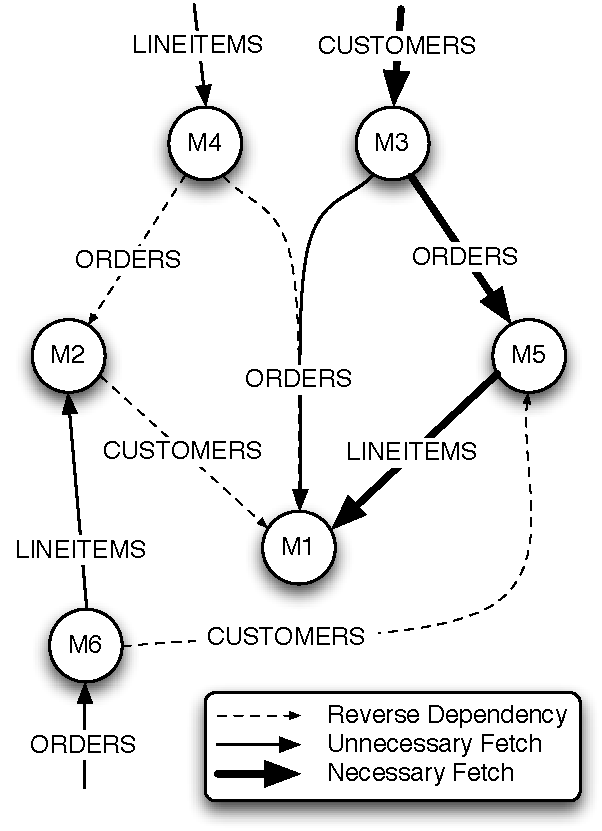
\includegraphics[width=2.5in]{images/q12_graph.pdf}
\caption{Data-flow graph for the example query.
Light and dashed edges can be eliminated.}
\label{fig:dataflow}
\end{center}
\end{figure}


When relations are joined along a key-foreign key relationship,
then we may assume that the transactional databases providing the updates
enforce their consistency. In particular, this means that we cannot use
a foreign key value until it has been inserted as a key; for instance, in
TPC-H, we cannot insert an order with a customer id for which there is
no customer; we first have to insert a suitable customer tuple.
Conversely, we cannot delete a customer until all its dependent orders
have been deleted.\footnote{Suitable code to implement ON DELETE CASCADE
semantics in M3 can be generated by compilation as well, but this is not
covered here because of lack of space.}
Because of lack of space, we only give an illustrative example which
is suggestive of the general algorithm.


\nop{
Thus, given key-foreign key joins, certain M3 statements that our compilation
algorithm produces are superfluous.
Consider a statement
{\tt foreach $\vec{y}$ do $m_2[\vec{x}\vec{y}]$ $\pm$= $t$}
in an on-insert trigger for relation $R$, .

These can be eliminated -- as an
optimization -- by analyzing the data flow graph of the program.
The nodes of this graph are the
map names of the M3 program and where there is an edge labeled $R$ from
node $m_1$ to $m_2$ if there is an M3 statement
{\tt foreach $\cdot$ do $m_2[\cdot]$ $\pm$= $t$} where
$m_1$ appears in $t$ in an insert or delete trigger for relation $R$.
Note that our compilation approach guarantees that this graph is always
acyclic (even if there are self-joins).
} % nop


\begin{example}\em
\label{ex:TPCH-Q12}
Consider the following query on a TPC-H like schema,
which counts the number of LineItems per customer id.
\begin{verbatim}
SELECT   C.cid, SUM(1)
FROM     Customer C, Order O, LineItem L
WHERE    C.cid=O.cid AND O.oid=L.oid
GROUP BY C.cid;
\end{verbatim}
Here, cid is a key for the Customer relation and oid is a key for the
Order relation, but oid is not a key for LineItem.
The compilation algorithm of Section~\ref{sec:compilation-alg} yields the
following insert triggers:
\begin{verbatim}
on insert into Customer(cid, nation) {
  q[cid] += qC[cid];
  foreach oid do qL[cid, oid] += qCL[oid, cid];
  qO1[cid] += 1
}
on insert into Order(oid, cid, ...) {
  q[cid] += qO1[cid]*qO2[oid];
  qC[cid] += qO2[oid];  qL[cid, oid] += qO1[cid];
  qCL[oid, cid] += 1;   qLC[oid, cid] += 1
}
on insert into LineItem(oid, ...) {
  foreach cid do  q[cid] += qL[cid, oid];
  foreach cid do qC[cid] += qLC[oid, cid];
  qO2[oid] += 1
}
\end{verbatim}

Consider the data flow graph for this program, which is shown in
Figure~\ref{fig:dataflow} and which illustrates the dependencies between
maps through updates to certain relations (the edge labels). All M3 statements
contributing dashed edges can be removed because these increments are zero unless a foreign key constraint is violated in the data. For example,
the statement {\tt q[cid] += qC[cid]} in {\tt on insert into Customer}
can be removed because {\tt qC} represents the number of line items for this
customer, and the customer is new. The solid thin lines represent
feasible updates to maps that have become disconnected from the query result
map, and can be eliminated.
The simplification yields the M3 program
\begin{verbatim}
on insert into Customer (cid, ...) { qO1[cid] += 1 }
on insert into Order (oid, cid, ...) {
  qL[cid, oid] += qO1[cid]
}
on insert into LineItem (oid, ...) {
  foreach cid do q[cid] += qL[cid, oid]
}
\end{verbatim}

The delete-triggers are precisely
like the insert-triggers, but with {\tt +=} replaced by {\tt -=}.
\punto
\end{example}





\section{The Cumulus System}
\label{sec:architecture}


\subsection{Architecture}


\begin{figure}
\hspace{-3mm}
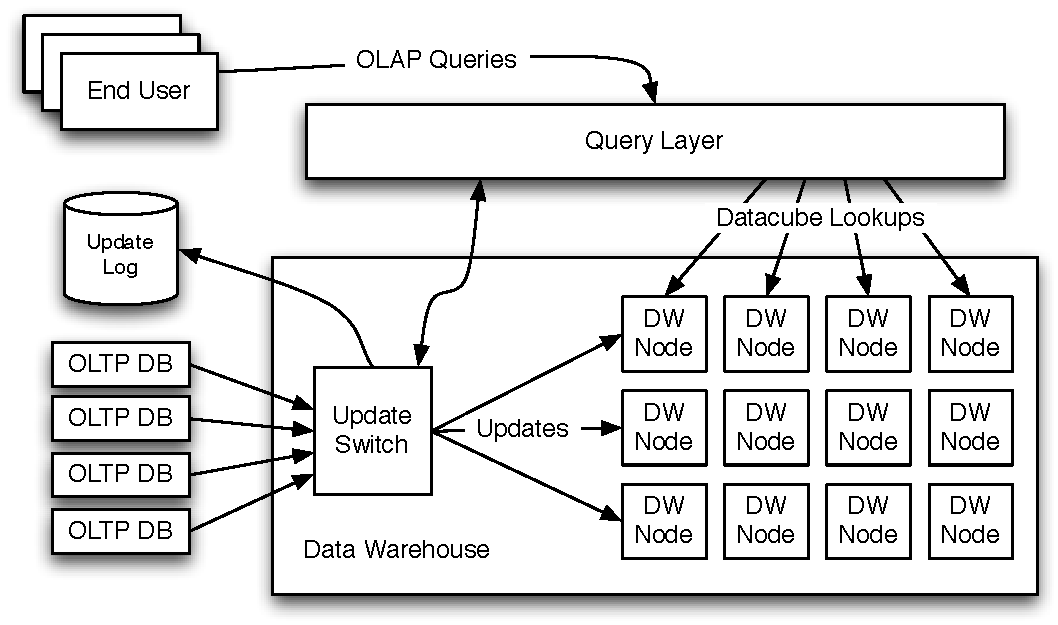
\includegraphics[width=3.4in]{images/Architecture.pdf}

\vspace{-4mm}

\caption{Cumulus' architecture.}
\label{fig:arch}
\end{figure}


Cumulus consists of three components: the compiler,
a {\em runtime}, and a {\em query layer}.
A diagram of this architecture is presented in Figure \ref{fig:arch}.

The compiler, which was discussed in the
previous section, translates SQL aggregation queries
into message passing programs that are executed by the runtime system.

The runtime accepts updates -- insertions and deletes of tuples --
at a coordinator node called the \textit{Switch}, which delegates
update work to a number of data storage and query processing nodes, or
\textit{DW Nodes}.
The maps suggested by the compiler -- and maintained by the M3 program --
are partitioned across the DW Nodes to keep network traffic to a minimum.  
The switch does not store any map data, but manages
the information about data placement (how maps are partitioned and which
partitions are located on which nodes).

The runtime is designed to implement exact online aggregation, and
we conceive it to be used for main-memory OLAP.
The query layer accepts roll-up/drill-down/slice/dice queries,
instructs the Switch to have the DW Nodes send a consistent version of
the relevant data to the querying node (the user's machine),
collects the result chunks there, and
finalizes the query answer
in a client-side API that runs on the user machine.

Our architecture supports the compilation of pre-aggrega\-tors close to the
OLTP database that reduce the load on Cumulus. For example, if sums of revenues
are to be computed, the revenues of batches of LineOrder tuples agreeing
on relevant join and group-by columns can be pre-aggregated close to the OLTP database and only this reduced workload of preaggregated tuples is sent to the Switch.

We generally assume that the data is persistent in the OLTP databases.
However, Cumulus is also able to
log the update stream arriving at the Switch and replay it from the
log later to recreate the data warehouse in main memory.
We could also log the map states using techniques as surveyed in
\cite{DBLP:journals/pvldb/SallesCSDGKW09}
for faster recovery, but this is currently not done.



\subsection{Data Placement}


The Switch maintains information how map data is partitioned across
DW Nodes. In the most general case, this would be a function
that maps a tuple update and a statement (id) from the M3 program to
a record that identifies, for each map access of the statement,
which DW Nodes store any relevant data for executing this
statement.
%
In the current prototype of Cumulus, maps are partitioned along
dimensional axes, akin to the partitioning done in grid files\cite{318586}.


\begin{example}\em
\label{ex:switch_msg}
Consider the M3 program of Example~\ref{ex:ssb}.
Assume there are nodes $N_1$ to $N_5$,
which store the following map partitions:
\begin{eqnarray*}
N_1 &:& mPL[*, \mbox{odd years}] \\
N_2 &:& mPL[*, \mbox{even years}], mDL[*, \mbox{green parts}] \\ 
N_3 &:& mDL[*, \mbox{red parts}] \\ 
N_4 &:& m[*, \mbox{odd years}] \\
N_5 &:& m[*, \mbox{even years}]
\end{eqnarray*}

Suppose {\tt on insert into Date($d_1$, 2005)} is triggered.
The trigger consists of only one statement,
{\tt mPL[datekey, year] += 1}, where datekey and year are instantiated
with $d_1$ and 2005, respectively. Since 2005 is odd,
the map values to be written are located on node $N_1$.
The statement contains no map values to be {\em read}.

For {\tt on insert into LineOrder($d_1$, $p_1$, $500$)},
there is one statement, which reads from $mPL$ and $mDL$ and writes to $m$.
The tuple ($d_1$, $p_1$, $500$)
does not provide useful information for restricting the nodes to be contacted
in this case.
Values of $m$ may be located on $N_4$ and $N_5$, values of $mPL$ may be
located on $N_1$ and $N_2$, and values of $mDL$ may be located on $N_2$ and
$N_3$.
\punto
\end{example}


\nop{
\begin{figure}
\begin{center}
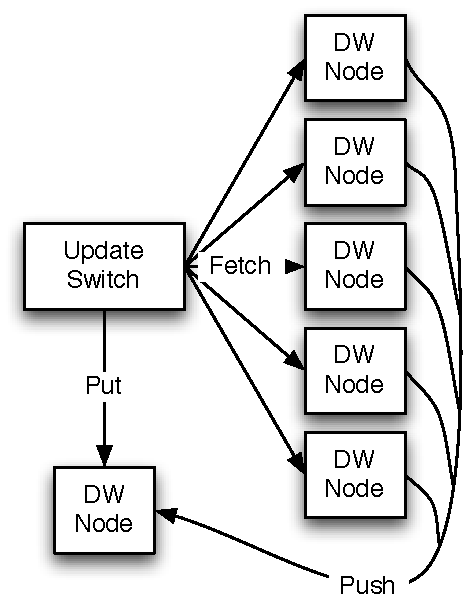
\includegraphics[width=1.5in]{images/UpdateStep.pdf}
\caption{Information flow during one map update.}
\label{fig:updatestep}
\end{center}
\end{figure}
} % end nop


\subsection{Update Protocol}


On an {\em update} (an insertion or deletion of a tuple
$\vec{x}\vec{y}$), an M3 program processes a set of statements of the form
\[
\mbox{{\tt foreach $\vec{z}$ do} $m[\vec{x}\vec{z}]$ += $t$
~~~~~or~~~~~ $m[\vec{x}]$ += $t$}
\]
in {\em arbitrary}\/ order.
%
Each update has a sequence number identifying it. All messages sent by the
Switch contain this update sequence number.

For a given statement, the Switch proceeds as follows.
It composes a set of messages parametrized on $\vec{x}\vec{y}$ and
dispatches them to the DW Nodes.
DW Nodes being read from are sent FETCH requests, which leads them to forward
PUSH messages containing the data read
to the appropriate writers. The writers are also
informed of their role by the Switch through PUT messages.

The update corresponding to an M3 statement is handled by the subset of
nodes that store partitions of the map being written to.  Each node
handles updates only for those partitions it stores locally. The Switch
uses the partition table to only contact readers who may store relevant information and writers who may have updates to do. 


As stated already, the nodes receiving a FETCH request perform the
requested reads and send their responses to the PUT nodes (the writers)
in a PUSH message.
The writers buffer received PUSH messages. For each write task to be
done, they receive a PUT message from the Switch which instructs them
what write to perform and which readers to expect PUSH messages from.
Readers who have received a FETCH message from the Switch always
send a PUSH message to the writers that were
identified by the Switch in the FETCH
message: If a reader has no relevant data, it sends an empty PUSH message to
the writer to allow it to move on.
This allows the writer to know when all necessary PUSH messages have been
received and the write can be carried out.

%An illustration of the complete message-passing process is given
%in Figure \ref{fig:updatestep}.  


\begin{figure}
\begin{center}
\begin{tabular}{l|r@{~}l}
to node & & message \\
\hline
$N_1$ & FETCH($t$, $s$, & push mPL[$d_1$, *] to $\{N_4\}$) \\[.7ex]
$N_2$ & FETCH($t$, $s$, & push mPL[$d_1$, *] to $\{N_5\}$ and \\
      &                 & push mDL[$p_1$, *] to $\{N_4, N_5\}$) \\[.7ex]
$N_3$ & FETCH($t$, $s$, & push mDL[$p_1$, *] to $\{N_4, N_5\}$) \\[.7ex]
$N_4$ & PUT($t$,   $s$, & {\tt foreach $(x,y)$ do} \\
      &                 & ~~{\tt m[$x,y$] += 500 * mDL[$p_1$, $x$]} \\
      &                 & ~~{\tt ~~~~~~~~~~~~~ * mPL[$d_1$, $y$]} \\
      &                 & with messages from $\{N_1, N_2, N_3\})$ \\[.7ex]
$N_5$ & PUT($t$,   $s$, & {\tt foreach $(x,y)$ do} \\
      &                 & ~~{\tt m[$x,y$] += 500 * mDL[$p_1$, $x$]} \\
      &                 & ~~{\tt ~~~~~~~~~~~~~ * mPL[$d_1$, $y$]} \\
      &                 & with messages from $\{N_1, N_2, N_3\})$
\end{tabular}
\end{center}

\vspace{-4mm}

\caption{Messages from the switch for Example~\ref{ex:switch_msg}.}
\label{fig:switch_msg}
\end{figure}



\begin{example}\em
\label{ex:switch_msg2}
We continue Example~\ref{ex:switch_msg} and take the partition choices
from there.
Suppose again that
{\tt on insert into LineOrder($d_1$, $p_1$, $500$)} is triggered and $t$ is
the sequence id of this update.
This trigger contains only one statement,
for which we generate an identifier $s$.
Then the switch sends the messages shown in Figure~\ref{fig:switch_msg}.
%
Let the current state of the maps be
mPL[$d_1$, 2005] = 1, mPL[$d_2$, 2006] = 1, mDL[$p_1$, red] = 1,
mDL[$p_2$, green] = 1. (These values are stored at nodes
$N_1$, $N_2$, $N_3$, and $N_2$, respectively).
Then the following PUSH messages will be sent:
\begin{center}
\begin{tabular}{ll|l}
from & to & message \\
\hline
$N_1$ & $N_4$ & PUSH($t$, $s$, mPL: $\{ [d_1, 2005] \mapsto 1 \}$) \\
$N_2$ & $N_4$ & PUSH($t$, $s$, mDL: $\emptyset$) \\
$N_2$ & $N_5$ & PUSH($t$, $s$, mPL: $\emptyset$; mDL: $\emptyset$) \\
$N_3$ & $N_4$ & PUSH($t$, $s$, mDL: $\{ [p_1, red] \mapsto 1 \}$) \\
$N_3$ & $N_5$ & PUSH($t$, $s$, mDL: $\{ [p_1, red] \mapsto 1 \}$) \\
\end{tabular}
\end{center}
\end{example}


In general, it is a goal of data placement
to partition maps in such a way that the number of
messages to be sent remains low. This can be done by collocating
corresponding partitions (via key-foreign key relationships)
of different maps on the same nodes.
In the previous example, the maps $m$ and $mDL$
could be partitioned on partkey and the partitions of $m$ and $mDL$ for the
same key ranges could be kept on the same nodes.
In the case of insertion of a LineOrder tuple, we would then know exactly
where to FETCH the mDL data; actually, this data would only have to be
PUSHed locally inside that node.


\subsection{Anatomy of a DW Node}


A DW Node receives and processes FETCH, PUSH, and PUT messages.
It has to process the messages it receives from the Switch 
in the order they are {\em sent}\/. For example, a
TCP connection with the Switch ensures that messages from the 
Switch do not arrive out of order. Apart from protocol messages
that ensure in-order delivery of FETCH and PUT messages, the Switch receives no
messages from the DW Nodes.
Incoming PUSH messages are buffered for inspection when it is the turn of
the corresponding PUT message to be processed.

\nop{
Internally, each DW Node maintains the current version
of the committed versions (identified
by update sequence numbers) of the maps it maintains. In practice, we
will only need to keep a relatively small number of versions, and we will always know when an old version is not needed anymore and an be dropped.
Since consecutive versions only have small differences, we maintain
old versions as diffs to the latest version.
} % end nop

The state of the DW Node includes, apart from a queue 
for the messages from the Switch and a buffer for PUSH messages, a
current update sequence number $t$ and a number
of map partitions that are stored and maintained at the node.
Conceptually, two versions of the map partitions are maintained,
one that represents a committed, consistent version of the data from the time after the
update with sequence number $t-1$ has been completed and before the update
of sequence number $t$ has started. This is the version from which FETCH
requests with update sequence number $t$ are served. The other
version is a working copy to which the writes of update sequence number
$t$ are applied.

The main thread of control processes the waiting messages from the Switch
in order.
For either a FETCH($t', s, \cdot$) or PUT($t', s,\cdot$) message, if its
update sequence number $t'$ is greater
than the local update sequence number $t$, then we set $t := t'$
and copy the working copy of the map partitions to the committed version.

Additionally,
for a FETCH message($t'$, $s$, push $m[\vec{\pi}]$ to $\textit{Ns}$),
we read the requested data $m[\vec{\pi}]$ from the committed version of
the map partitions and send it in PUSH messages to the set of recipient
nodes $\textit{Ns}$.

For a message PUT($t'$, $s$, $st$ with messages from $\textit{Ns}$), where $st$
is an M3 statement and $s$ the identifier used for it throughout the 
system, we block until all PUSH messages have arrived for all
senders announced in set $\textit{Ns}$.
Let $m_1[\vec{t}_1]$, $\dots$, $m_k[\vec{t}_k]$ be the map accesses occuring in
$st$. For each $m_i$, 
we extract the data from the PUSH messages corresponding
to the current PUT message (i.e., agreeing on $t'$ and $s$) and put it in a table $T_i$.
If $\vec{t}_i$ consists of constants only (i.e., does not contain any
of the variables that the optional foreach loop loops over), and $T_i$ is
empty, then we have to compute an inital value for
$m_i[\vec{t}_i]$.\footnote{Currently,
the DW Nodes do not (but the compiler does) support $<$/$\le$-join conditions,
and the M3 programs produced guarantee that the map value must be 0.}
For each tuple of the product table $T_1 \times \dots \times T_k$,
we evaluate $st$ and perform one map update.
If $st$ does not contain a foreach-loop, then each $T_i$ contains exactly
one value, and we update exactly one map value.


\begin{example}\em
\label{ex:switch_msg3}
We continue Example~\ref{ex:switch_msg2}.
Node $N_4$ knows from the message
\begin{center}
\begin{tabular}{ll}
PUT($t$,   & {\tt foreach $(x,y)$ do} \\
           & ~~{\tt m[$x,y$] += 500 * mDL[$p_1$, $x$]} \\
           & ~~{\tt ~~~~~~~~~~~~~ * mPL[$d_1$, $y$]} \\
           & with messages from $\{N_1, N_2, N_3\})$
\end{tabular}
\end{center}
that it has received from the Switch
that it will receive messages with timestamp $t$ from nodes $N_1$, $N_2$, and
$N_3$.
The information it receives in these three PUSH messages is
$T_{mDL} = \{ [p_1, red] \mapsto 1 \}$ and
$T_{mPL} = \{ [d_1, 2005] \mapsto 1 \}$.
Thus, $N_4$ executes the update
{\tt m[red, 2005] += 500 * 1 * 1}
on the working copy of $m$. 
\punto
\end{example}



\newcommand{\figurewidth}[0]{1.8in}

\newcommand{\tablefig}[1]{
  \hspace*{-0.25in}
  \includegraphics[width=\figurewidth]{../graphs/graphs/#1}
}

\begin{figure}
\begin{center}
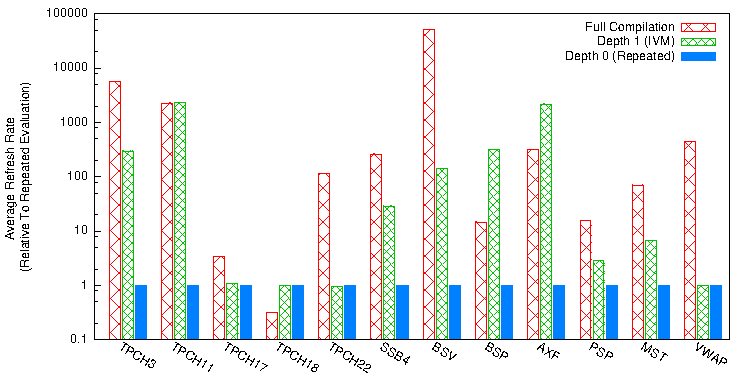
\includegraphics[width=3.4in]{../graphs/graphs/bakeoff.pdf}
\caption{Cross-query comparison of our compiler in different depth-restricted modes, and the best performing streaming and database engine for each query.  Note the logscale on the y-axis.}
\label{fig:experiments:bakeoff}
\end{center}
\end{figure}

\begin{figure*}
\begin{center}

\begin{minipage}{\textwidth}
\begin{center}
\hspace*{0.1in}
\begin{tabular}{cccc}
\tablefig{unified_tpch3.pdf} &
\tablefig{unified_tpch11.pdf} &
\tablefig{unified_tpch17.pdf} &
\tablefig{unified_ssb4.pdf} \\
(a) & (b) & (c) & (d)
\end{tabular}
\caption{TPC-H Query 3~(a), 11~(b), 17~(c), and SSB4~(d): (a) By the 40\%\ marker, all streams except LINEITEM have completed, and the remaining tuples consume no additional memory. (b) For simple two-way joins, full compilation is virtually identical to depth 1. (c) Due to the nested aggregate, IVC requires a nested loop, while full compilation requires only a single scan.(d) Full compilation is a full polynomial order faster than in IVC, although performance does begin to drop once the system begins running out of memory around the 27\%\ marker.}
\label{fig:experiments:tpch3}  
\label{fig:experiments:ssb4}
\label{fig:experiments:tpch17}
\label{fig:experiments:tpch11}
\end{center}
\end{minipage}

\vspace*{0.2in}

\begin{minipage}{\textwidth}
\hspace*{0.1in}
\begin{tabular}{cccc}
\tablefig{unified_brokervariance.pdf} & 
\tablefig{unified_tpch22.pdf} &
\tablefig{unified_vwap.pdf} &
\tablefig{unified_serverload.pdf} \\
(a) & (b) & (c) & (d)
\end{tabular}
\caption{BSV~(a), TPC-H Query 22~(b), VWAP~(c), and SVL~(d):  (a) The many-to-many relationship on the join term forces IVM to perform linear work on each insertion, which full compilation avoids.  (b) The small CUSTOMER stream completes at the 10\%\ marker, while the remaining ORDERS tuples require only linear time with full compilation. (c) IVM repeatedly re-evaluates the nested (parameterized) sub-query, while full compilation maintais a cache of sub-query results. (d) Materializing nested queries gains a polynomial degree of performance over IVM, but memory continues to grow. }
\label{fig:experiments:brokervariance}
\label{fig:experiments:tpch22}
\label{fig:experiments:vwap}
\label{fig:experiments:serverload}
\end{minipage}

\vspace*{0.2in}

\begin{minipage}{\textwidth}
\hspace*{0.1in}
\begin{tabular}{cccc}
\tablefig{unified_pricespread.pdf} &
\tablefig{unified_missedtrades.pdf} &
\tablefig{unified_axfinder.pdf} &
\tablefig{unified_brokerspread.pdf} \\
(a) & (b) & (c) & (d)
\end{tabular}
\caption{PS~(a), MST~(b), AXF~(c) and BSP~(d):  (a,b) The performance and memory plateaus result from a portion of the trace from about 0.001\%\ to 0.01\%, where a single order is repeatedly placed and revoked. (c,d) Full compilation's aggressive materialization strategy results in the caches growing too large to be efficiently maintained.}
\label{fig:experiments:pricespread}
\label{fig:experiments:MST}
\label{fig:experiments:axfinder}
\label{fig:experiments:brokerspread}
\end{minipage}



\end{center}
\end{figure*}

\begin{figure*}
\begin{center}

%\begin{minipage}{\textwidth}
%\begin{center}
%\begin{tabular}{ccc}
%(a) & (b) & (c)
%\end{tabular}
%\caption{TPC-H Query 18~(a). }
%\label{fig:experiments:tpch18}
%\end{center}
%\end{minipage}
%
\vspace*{0.1in}

\begin{minipage}{\textwidth}
\begin{center}
\begin{tabular}{cccc}
\tablefig{unified_tpch18.pdf} &
\tablefig{unified_5gig_tpch3.pdf} &
\tablefig{unified_5gig_tpch11.pdf} &
\tablefig{unified_5gig_tpch22.pdf} \\
(a) & (b) & (c) & (d)
\end{tabular}
\caption{TPCH Query 18 (a): An incorrectly chosen join ordering prevents full compilation from effectively exploiting foreign key dependencies in the TPC-H schema;  The three fastest-running TPC-H queries (3~(b), 11~(c), and 22~(d)) run on a 5GB dataset: (b) Quadratic effects from early parts of the workload become apparent in IVM at this scale, while full compilation remains linear. (c) Maintaining the base relations already projected and aggregated gives a slight edge to full compilation at this scale.  (d) Full compilation performance is reduced due to updates being linear in the size of CUSTOMER, but still performs better than depth 1.}
\label{fig:experiments:big}
\label{fig:experiments:big:tpch3}
\label{fig:experiments:big:tpch11}
\label{fig:experiments:big:tpch22}
\end{center}
\end{minipage}

\end{center}
\end{figure*}

We now analyze the performance of our compilation techniques.  As in Section \ref{sec:dbfail}, our experiments are run on Redhat Enterprise Linux running in a VM with 16 GB of RAM, and 2x4 core Intel Xeon E5620 2.4 GHz processors allocated to it.  Note that our compiler produces single-threaded code, while other platforms were allowed to consume the full resources of the VM.

Our analysis uses the same queries and methodology as in Section~\ref{sec:tscomparison}: The queries are described in Section~\ref{sec:tscomparison:workload}, and expressed in SQL form in Appendix~\ref{app:queries}.

% we analyze our compiler's performance on TPC-H\cite{tpch} Queries 3, 11, 17, 18, and 22, a variant of Star Schema Benchmark\cite{ssb} Query 4 six orderbook queries: VWAP, PS, MST, AXF, BSP, and BSV, and a cluster monitoring query: SVL.  TPC-H queries were modified slightly due to a lack of support for certain advanced features in our SQL parser (e.g., Having, Exists, etc...).  SQL for the queries in our test workload is presented in Appendix

%Our analysis uses the queries from Examples \ref{ex:dbfail:stock} (PS),  \ref{ex:dbfail:tpch} (SSB4), and \ref{ex:dbfail:network} (SVL), Queries numbers 3, 11, 17, 18, and 22 from the TPC-H\cite{tpch} benchmark, the VWAP query presented in \cite{kennedy-ahmad-koch-cidr:11}, and four additional financial queries: MST, AXF, BSP, and BSV in the spirit of VWAP and PS.  The structure of these queries is discussed below.

Queries were run on pre-generated traces until completion of the trace or a 1 hour cutoff was reached.  Traces were generated as follows: The queries: VWAP, MST, AXF, BSP, PS, and BSV were run on a 2.63 million tuple trace of an order book update stream, representing of one day of stock market activity for MSFT.  BID and ASK orders (and cancellations) were translated into equivalent operations on a BIDS and ASKS table, with tuples in either table comprised of a timestamp, an order id, a broker id, a price, and a volume.  The broker id was synthesized for each order -- our experiments use 10 brokers, assigned deterministically based on the order id.  The stream consists of approximately 1.4 million operations on the BIDS table, and 1.14 million operations on the ASKS table.

Queries based on the TPC-H schema (including SSB4) were run on a scaling-factor 0.1 (100 BM) database generated by dbgen\cite{tpch}.  Additional scaling experiments were carried out on TPC-H queries 3 and 11 at scaling factors 0.5, 1, 5, and 10 -- these results are presented in Section~\ref{sec:experiments:bigds}.  Insertions are drawn in-order from each output file of dbgen, with rows from different tables interleaved in random order.  Note that it possible for rows to be inserted before a foreign key constraint has been satisfied, and that smaller datafiles will finish earlier in the stream.  This is not expected behavior in a streaming setting, but provides valuable insights about the performance characteristics of insertions into different tables.

SVL was run on a synthetically generated dataset, simulating 1000 racks of 20 servers each, emitting a total of 100,000 state updates.  The first 20,000 operations in the trace consist of an insertion for each server at 0 load.  For each state update, a random server deletes its previous state tuple and inserts a tuple declaring its new load -- a random real between 0 and 1.

Figure \ref{fig:experiments:bakeoff} compares recursive compilation to the performance of traditional databases and stream processors -- results presented overlap with those of Figure~\ref{fig:queries}.  These numbers speak for themselves, but clearly, traditional engines are not designed for our problem domain.

In order to evaluate our compilation algorithm in a fair environment with a common baseline for performance, we use a depth-limited instantiation of our compilation algorithm: Instead of recursively computing the entire materialization plan, the compiler stops after a fixed number of recursive steps.  Beyond this stage, queries are not materialized and instead computed directly from the base relations.

Compilation at depth-1 is equivalent to traditional IVM techniques, and depth-0 is equivalent to re-evaluating the query on every insertion.  We omit detailed depth-0 performance measurements on graphs where these results are not visible due to scale, or where depth-0 and depth-1 performance are indistinguishable.  Memory measurements are taken using google-perftools\cite{perftools}, and count only memory allocated to the persistent maps and not transient datas (e.g., materialized join results).

As a consequence of the high join width of SSB4, the default materialization plan has an extremely high branching factor (12 at the top level).  Although most materialized views in the plan are duplicates, the compiler must still explore all children of unique nodes -- a prohibitively expensive process.  For the purpose of these experiments, we omit deletions when compiling SSB4 (halving the branching factor).  As SSB4 is a query without nested aggregates, deletions are symmetric with insertions -- In spite of the prohibitive compilation time, the behavior of the compiled query is identical.

\subsection{Equijoins}

We first analyze the performance of our compiler on three equijoin queries with no nested aggregates.  Our compiler recurs only once on TPC-H Query 11.  As a consequence, the result is nearly equivalent to IVM\footnote{We pre-aggregate the materializations of SUPPLIER and PARTSUPP, but this provides only a minor improvement at this scale due to the bounded fanout of this query.}.  

Both TPC-H Query 3 and SSB4 demonstrate a substantial performance increase over IVM.  The one-to-one, and bounded fanout one-to-many relationships between elements of many of these queries are actually advantageous to the IVM implementation -- each insertion only triggers a limited number of reads.  In spite of this, incrementally maintaining the (aggregate) delta queries results in a net reduction in the amount of work required -- especially in a large query like SSB4.

Also note the memory usage of TPC-H Query 3.  Starting by the 40\%\ marker, all streams have been exhausted except for LINEITEM.  The final aggregate's group-by columns are drawn purely from the order table, so insertions into LINEITEM only update aggregate values that have already been allocated by the corresponding ORDER.  Thus, memory usage plateaus for full compilation, while the IVM implementation must continue to store each row.

This is not always true.  For extremely large queries like SSB4 (a 7-way join), the number of intermediate materialized views created is quite large.  Despite the large amount of state that the fully compiled query maintains, any individual update modifies only a small amount of that state, and the fully compiled query's efficiency is unaffected as long as the system has enough memory.  However, memory usage is an important part of the cost/benefit tradeoff of full compilation -- We address a broader range of materialization strategies below in Section~\ref{sec:experiments:othermetrics}.

\subsection{Nested Subqueries}

Figures \ref{fig:experiments:tpch17}c, \ref{fig:experiments:tpch22}b, and \ref{fig:experiments:vwap}c illustrate the performance of our compiler on several queries with nested aggregates.

The lookup over ORDERS in TPC-H Query 22 can be evaluated in constant time both using IVM and full compilation.  However each insertion into ORDERS requires evaluation of the nested aggregate on CUSTOMER, while full compilation maintains a materialized instance of this.

while this value is materialized by the fully compiled version.


queries the CUSTOMER table with two selection conditions: a comparison based on an uncorrelated nested aggregate query over CUSTOMER, and a second based on a lookup (an EXISTS) on ORDERS.   .  

In IVM, insertions into CUSTOMER depend on whether the query optimizer detects that the nested aggregate is uncorrelated and computes it before the rest of the query.  If not, the insertion requires quadratic work, and even if it does, each insertion requires two complete iterations over the customer table: once to compute the aggregate and once to figure out for which customers the state of the comparison changes.  This latter iteration can not be eliminated by full compilation, but the iteration is only over those rows already known to satisfy the selection condition on ORDERS.

VWAP is a query over BIDS with two selection predicates: one over an uncorrelated nested aggregate over BIDS, and one over a correlated (via inequality on the price from the outer BIDS table) nested aggregate over BIDS.  As in TPC-H Query 22, whether the uncorrelated aggregate is an issue for IVM is dependent on the query optimizer.  

The inequality-correlated aggregate is of more interest here.  Because the domain of the correlating variable (price) is determined outside the nested aggregate, the nested subquery must be re-evaluated every time a new price is encountered.  However, the resulting value can then be stored and incrementally maintained.  The domain of prices is bounded, so after an initial ramp up process (that occurs while the size of the table is small) the fully compiled version can incrementally maintain the query output in (close to) constant time.

BSV (Figure \ref{fig:experiments:brokervariance}a) is a two-way aggregate self-equi-join over BIDS.  Despite the lack of a nested aggregate, the performance of BSV follows a pattern similar to the prior two queries.  This is not surprising -- correlated aggregate subqueries are known to be equivalent\todo{cite?} to joining the result with a group-by aggregate query.  Thus, materializing a nested aggregate is tantamount to materializing the first delta.  Furthermore, unlike TPC-H Query 11 (Figure \ref{fig:experiments:tpch11}d), the join relationship is many-to-many, and the benefits of maintaining the join result as an aggregate grow over time.

TPC-H Query 17 is a two-way equi-join over PART and LINEITEM with a correlated nested aggregate over LINEITEM.  Both the join and the correlation are on partkey.  As in the prior queries in this section, incrementally maintaining the nested aggregate makes insertions into PART constant-time rather than linear.  However, even in the fully compiled query, insertions into the LINEITEM table must still iterate over all matching results in the join, which are already being materialized.  

\subsection{5 GB Dataset}
\ref{sec:experiments:bigds}
Figure \ref{fig:experiments:big} presents the behavior of the three fastest TPC-H queries on a scaling factor 5 (5 GB) database.

In the IVM version of TPC-H 3, the one-to-many relationship between them makes each insertion into CUSTOMER linear in the number of LINEITEMS matching CUSTOMER (an average fanout of 40).  A small CUSTOMER table can be processed before many ORDERS are inserted.  With the larger dataset, the increasing cost of insertions into CUSTOMER becomes more pronounced, while the fully compiled version remains constant-time throughout.

Although IVM is nearly identical to full compilation on TPC-H 11, full compilation pushes aggregation into the materialized view while IVM performs the aggregation at lookup.  This, when inserting into SUPPLIER, full compilation reads precisely one value, while IVM reads approximately 80 (and must aggregate over them).  IVM stores both base relations in their entirety, while full compilation stores only the subset needed for query maintenance.  As a consequence, full compilation has a constant, but visible improvement in both performance and memory use at this scale.

Under full compilation, TPC-H Query 22 requires a linear amount of work for insertions into CUSTOMER and a constant amount of work for insertions into ORDERS.  On the small dataset, full compilation was able to get through the CUSTOMER table (note the quadratic behavior in Figure \ref{fig:experiments:tpch22} up to about the 18\% marker) and quickly completed the much larger ORDERS table.  On the larger dataset, full compilation gets bogged down in processing CUSTOMER.

\subsection{Limited Recursion}
\label{sec:experiments:othermetrics}

\begin{figure*}
\begin{center}
\begin{tabular}{|l|c|c|c|c|c|c|}\hline
{\bf Depth} & 1 & 2 & 3 & 4 & 5 & Full \\ \hline 
Avg Rate (refreshes/s) & 5.91 & 0.373 & 0.7 & 12.7 & 51.5 & 50.4 \\ \hline 
Avg Memory per Tuple & 98.5 B & 0.0 B & 0.0 B & 0.0 B & 0.0 B & 61.0 KB \\ \hline 
Lines of Code & 3174 & 12015 & 16517 & 13215 & 10998 & 10431 \\ \hline 
Number of Maps &        6 &       18 &       36 &       45 &       45 &       39 \\ \hline 
\end{tabular}
\caption{Statistics for different compilation depths on SSB4.  Depth-5 is equivalent to full compilation, but also maintains copies of each of the 6 base relations.}
\label{fig:experiments:ssb4depth}
\end{center}
\end{figure*}
We now explore the space of limited recursive compilation beyond IVM.  Figure \ref{fig:experiments:ssb4depth} illustrates the effects of limiting compilation to depths between 0 and 5.  Recall that the maximum recursive depth is one less than the join width of the query.  Thus for SSB4 (which has a join width of 6), compilation to depth-5 is equivalent to full compilation, save that the base relations are maintained and materialized.

At depth-1, the compiled query materializes only the base relations and no intermediate tables.  It must still perform a 5-way join on every insertion, but  only once per update.  The 6 materialized views that it maintains are the 6 base relations from the query.  

At depth-2, the compiled query must now maintain 12 intermediate materialized views, several of which require (effectively) a 4-way join to maintain.  The net cost of maintaining these additional maps does not begin to pay off until depth-4 (where maintenance operations are reduced to at most 2-way joins).  By this point, decomposition has already resulted in the instantiation of all intermediate materializations relevant to the query, so extra and unnecessary work is being done.  

The effectiveness of this approach at depth-4 (in spite of the extra work being done) suggests that a more effective approach to reducing memory consumption might be to materialize not just the set of views closest to the root, but rather a subset of the entire materialization plan (e.g., requiring at most two-way joins throughout the materialization plan).  However, there exists an incredibly large space of possible materialization plans ($2^{39} \approx $ half a trillion possibilities for SSB4) -- cost based optimization within the space of possible materialization plans is future work.

\subsection{Functional Optimizations}
\todo{Yanif}

\subsection{Memory, Extraction, and Future Work}
\label{sec:experiments:future}

\begin{figure}
\begin{center}
\begin{tabular}{|l|c|c|c|}\hline 
\ & Infinite Depth & Depth 1 & Depth 0 \\\hline 
TPCH3 & 2509 & 2855 & 4198 \\\hline
TPCH11 & 531 & 596 & 616 \\\hline
TPCH17 & 928 & 1158 & 1478 \\\hline
TPCH18 & 3668 & 3538 & 4631 \\\hline
TPCH22 & 777 & 1135 & 754 \\\hline
SSB4 & 10995 & 8954 & 7904 \\\hline
BSV & 342 & 327 & 347 \\\hline
BSP & 45625 & 567 & 729 \\\hline
AXF & 2169 & 553 & 1394 \\\hline
PSP & 1442 & 1878 & 1890 \\\hline
MST & 5457 & 2870 & 2434 \\\hline
VWAP & 533 & 466 & 341 \\\hline
\end{tabular}
\caption{Lines of Code Per Query}
\label{fig:experiments:loc}
\end{center}
\end{figure}

It is important to understand not only where our compiler succeeds, but where its limitations lie.  We now consider several cases where the observed performance of our technique does not match up with our (high, and perhaps naive) expectations.  As a consequence of our experimentation and analysis, we have identified three core challenges for future work in this area.

\tinysection{Join Ordering}
The first case of poor performance we consider is TPC-H Query 18 (Figure \ref{fig:experiments:tpch18}a), a three-way join over CUSTOMER, ORDERS, and LINEITEM, with an EXISTS predicate over a query that itself has a nested aggregate as a condition.  Although the query effectively involves two levels of nesting, it is otherwise quite simple.

Yet in spite of the simplicity, the query performs badly -- the query performs better at depths 0 and 1.  The reason for this poor performance is our join ordering heuristic: The trigger that updates the query result must compute a join between the delta of the extracted nested subquery (aggregated over orderkey) and a materialized representation of CUSTOMER $\bowtie$ ORDER $\bowtie$ LINEITEM (aggregated over custkey and orderkey).  

Not knowing about the one-to-many relationship between custkey and orderkey, we iterate over the materialized join first and effectively iterate over all orders placed so far.  Join ordering is a well studied problem in the database community, and the solution to this problem is purely an engineering challenge.  A further unfortunate side effect of the incorrect join ordering is that the added (unnecessary) looping involves lookups that extend the domain of several intermediate materialized views, causing an explosion of memory use.

\tinysection{Domain Maintenance}
The second case is best illustrated by SVL (Figure \ref{fig:experiments:serverload}d), a query over a single SERVERS table with a single selection predicate based on two uncorrelated aggregates.  By all rights, this query should perform as well as TPC-H Query 22, VWAP, and BSV (Figure \ref{fig:experiments:tpch22}).  The difficulty here is related to domain maintenance \todo{Do we discuss this elsewhere in the paper?  Backreference... this is not the place to be discussing it}.  In effect, our runtime is unable to properly garbage collect deleted entries in one of the materialized views, resulting in a progressively growing workload on every insertion.  

A similar issue affects both PS and MST (Figures \ref{fig:experiments:pricespread}a, and \ref{fig:experiments:missedtrades}b respectively), both two-way joins over BIDS and ASKS.  In both queries there are two selection predictaes: one comparing a column of ASKS to nested subquery over ASKS, and a similar predicate over BIDS.  Apart from a stretch of updates (0.001\%\ to 0.01\%\ in the trace) in the stock market trace where the same order is repeatedly placed and revoked the query performance follows a very similar performance curve. 

\tinysection{Map Extraction}
The final case of performance issues is seen in both AXF (Figure \ref{fig:experiments:axfinder}c) and BSP (Figure \ref{fig:experiments:brokerspread}d), both simple two-way inequality joins.  Our aggressive extraction heuristic attempts to materialize the entire delta query, which for inequality joins includes an unbound variable.  In such cases, the extracted expression is incrementally maintained for every encountered valuation of the unbound variable.  Thus, each change to the extracted expression requires an iteration over all previously encountered values.  In most cases, most of the state kept for each row in this output can be pre-aggregated and is typically quite small.  However, in the case of these two queries, these tables are each approximately the size of both input tables.  An improved, data-dependent extraction heuristic could identify such situations and compute the inequality join inline -- effectively doing what IVM does.  Alternatively, the entire materialized delta could be incrementally maintained more efficiently using datastructures suited to computing aggregates over ranges (e.g., \cite{range trees}).

\tinysection{Summary}
Our compilation technique is effective on select-project-join-aggregate queries involving equi-joins and nested subqueries which are uncorrelated, correlated through an equality comparison, or correlated on a variable (or variables) with a small domain.  It is especially good on queries with small result sets (but large inputs).

Our technique is less effective on inequality joins and nested aggregates correlated through an inequality -- although both are still handled efficiently if the domain of the values being compared is small.  In a similar vein, we do not optimize to take advantage of, or avoid problems caused by data-specific characteristics (e.g., foreign keys, large domains, etc\ldots). 



\begin{figure}
\begin{center}
\end{center}
\end{figure}






\section{Related Work}
\label{sec:relatedwork}


Database compilers \cite{DBLP:conf/pods/Batory88,DBLP:journals/jiis/BatoryT97}.

Data cubes \cite{datacube}.
Online aggregation (that is, by approximation --
\cite{DBLP:conf/sigmod/HaasH99, DBLP:conf/sigmod/RusuXPWJJD08, DBLP:conf/sigmod/AcharyaGPR99}).

A large body of previous research has focused on incremental view maintenance
of relational database queries. The
focus of this work was always on only one level of delta rewriting
and then using classical relational query processing techniques
based on interpreted query plans and heavyweight monolithic query operators
(such as joins).
In general, however, this means
that the rewritten query is still an arbitrarily complex query (in the number
of joins) and the message passing technique employed in Cumulus is not
applicable.

Most of the previous work on incremental view maintenance does not observe or leverage the fact that aggregation in queries can actually make incremental maintenance {\em easier}, rather than harder, because it greatly reduces the amount of data in the result and because numbers have additional algebraic properties that relations do not have and which allow for further decomposition and optimization of queries.

Column stores \cite{DBLP:journals/tods/Batory79,DBLP:conf/cidr/KerstenM05,DBLP:conf/vldb/StonebrakerMAHHH07}
are a prominent and successful instance of the recent trend
to abandon rather old database technologies and try out new architectural
para\-digms. Column stores have also been shown to be particularly well suited
for OLAP. However, column stores are fundamentally a secondary storage
concept; in main memory, it does not seem to be particularly meaningful to talk of column or row stores. To date, there has also been no work
on incremental view maintenance in column stores.
Indeed, they are notoriously bad at updating (worse than classical row stores).

\nop{
H-Store is an OLTP system that abandons classical concurrency control and
recovery baggage for very high performance. It is interesting for the
fresh look at things, and for the viewpoint that even OLTP systems should
be much simpler, nimbler systems than classical databases, which is also
part of the vision behind Cumulus. However, H-Store solves a problem very
different from the one addressed by Cumulus.

Recently, a number of startups have taken off with the idea of running
databases -- even classical technology such as Postgres -- in the cloud
(e.g. Greenplum and Aster Data). While several systems aim at OLAP
applications, none of them allows for true online aggregation as Cumulus does,
and none of the systems takes as radical a lightweight, systemsy approach
as Cumulus.
} % end nop



\section{Conclusions}
\label{sec:conclusions}


How do we partition data (the layout)?  Where do various bits of code get executed live?  What kind of runtime analytics do we need to collect to manage the data layout on the fly? 



\bibliographystyle{abbrv}
\bibliography{main}


%\newpage


\appendix

\section{Further Examples}


A second example for the foreign-key optimization:


\begin{example}
Consider again Example~\ref{ex:ssb}:
\begin{verbatim}
SELECT   P.partcat, D.year, SUM(revenue)
FROM     Date D, Part P, LineOrder L
WHERE    D.datekey=L.datekey
AND      P.partkey=L.partkey
GROUP BY P.partcat, D.year;

+Date(datekey, year):
 (partcat: Part.partcat)
    m[partcat, year] += mD[datekey, partcat];
 (partkey: Part.partkey)
    mP[partkey, year] += mDP[datekey, partkey];
 mPL[datekey, year] += 1

+Part(partkey, partcat):
 (year: Date.year)
     m[partcat, year] += mP[partkey, year];
 (datekey: Date.datekey)
    mD[datekey, partcat] += mDP[datekey, partkey];
 mDL[partkey, partcat] += 1

+LineOrder(datekey, partkey, revenue):
 (partcat: Part.partcat, year: Date.year)
  m[partcat, year] += revenue
    * mPL[datekey, year] * mDL[partkey, partcat];
 (partcat: Part.partcat) mD[datekey, partcat] +=
    revenue * mDL[partkey, partcat];
 (year: Date.year) mP[partkey, year] +=
    revenue * mPL[datekey, year];
 mDP[datekey, partkey] += revenue;


on insert into Date (datekey, year) {
 mPL[datekey, year] += 1
}
on insert into Part (partkey, partcat) {
 mDL[partkey, partcat] += 1
}
on insert into LineOrder
           (datekey, partkey, revenue) {
  (partcat: Part.partcat, year: Date.year)
  m[partcat, year] += revenue
                    * mPL[datekey, year]
                    * mDL[partkey, partcat]
}
\end{verbatim}
\end{example}


%\section{Figures}


\begin{figure}
\begin{center}
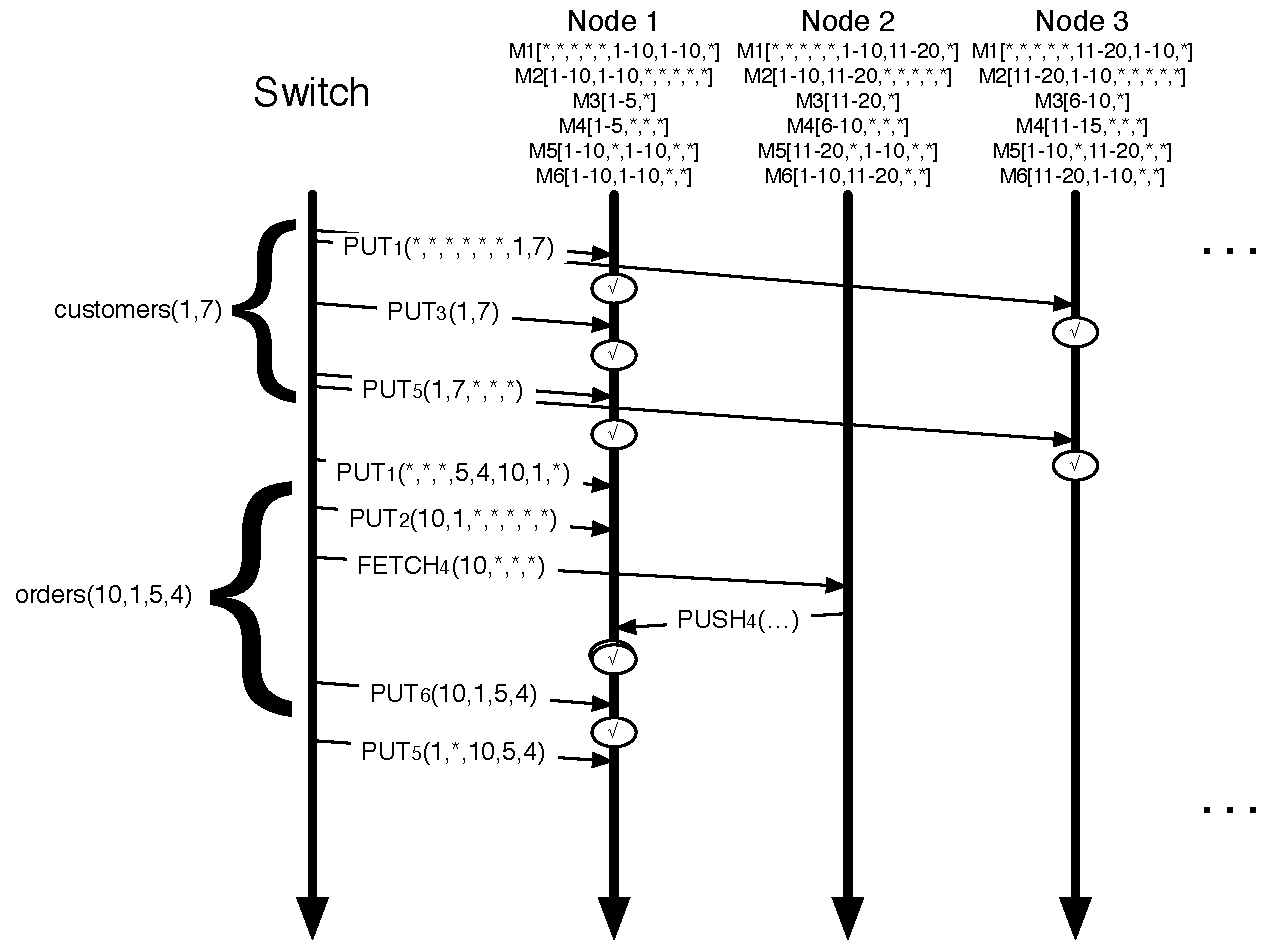
\includegraphics[width=3.5in]{images/MessageFlow.pdf}
\caption{Sequence diagram.}
\end{center}
\end{figure}




\end{document}  
